%!TEX program = xelatex
\documentclass[a4paper,12pt]{report}
\usepackage[left=3cm, right=2.5cm, top=2.3cm, bottom=3.5cm]{geometry}
\usepackage{amsmath}
\usepackage{mathtools}
\usepackage{amsfonts}
\usepackage{amssymb}
\usepackage[ruled,linesnumbered]{algorithm2e}
\newcommand\mycommfont[1]{\footnotesize\ttfamily\textcolor{blue}{#1}}
\SetCommentSty{mycommfont}
\usepackage{graphicx}
\usepackage{subfig}
\usepackage{caption}
\usepackage{enumerate}
\usepackage{titlesec}
\usepackage{url}
\usepackage{color}
\usepackage{tabu}
\usepackage{makecell}
\usepackage[table]{xcolor}
\usepackage[T1]{fontenc}
\usepackage{enumitem}
\usepackage{cite}
\usepackage[redeflists]{IEEEtrantools}
\usepackage{fancyhdr}

\renewcommand{\baselinestretch}{1.5}
\parindent=0pt
\titleformat{\chapter}[block]{\LARGE\bfseries}{\chaptertitlename\ \thechapter}{1em}{\LARGE}
\graphicspath{ {./images/} }

\title{Hierarchical Indoor Positioning System Based on Wireless Signals and Images in Dynamic Indoor Environment}
\author{Student: Meng-Ni Hsieh \\
Advisor: Prof. Sok-Ian Sou \\
\\
Department of Electrical Engineering  \\
College of Electrical Engineering and Computer Science \\
National Cheng Kung University \\
Thesis for Master of Science Degree \\
}
\date{June, 2023}

\allowdisplaybreaks[1]

% 為 titlepage 添加頁碼
% \fancypagestyle{titlepagestyle}{
%   \fancyhf{} % 清空頁眉頁腳
%   \pagenumbering{roman}
%   \setcounter{page}{2}
%   \cfoot{\thepage} % 在中央位置顯示頁碼
%   \renewcommand{\headrulewidth}{0pt} % 移除頁眉的分隔線
% }


\begin{document}
% \bstctlcite{IEEEexample:BSTcontrol}
\maketitle
\begin{titlepage}
% \thispagestyle{titlepagestyle} % 為 titlepage 添加頁碼
    \begin{center}
        {\bf\large Hierarchical Indoor Positioning System Based on Wireless Signals and Images in Dynamic Indoor Environment}\\
        {Postgraduate: Meng-Ni Hsieh \hspace{8mm} Advisor: Prof. Sok-Ian Sou}\\
        {Department of Electrical Engineering}\\
        {College of Electrical Engineering and Computer Science}\\
        {National Cheng Kung University}\\
    \end{center}

    \paragraph{}
    \begin{center}
        {\bf Abstract}
    \end{center}
    \paragraph{}
    Nowadays, mobile devices are equipped with wireless signal modules and built-in cameras, making it easy to leverage these resources for indoor positioning. Many research studies integrate these two complementary types of data using a hierarchical framework to address the limitations of relying solely on a single data source for positioning. However, hierarchical architectures heavily rely on the coarse-grained positioning results, and existing research often uses only one type of data for coarse-grained positioning, which may compromise the reliability of this stage. Therefore, we propose a hierarchical indoor positioning system that combines wireless signal and image data. In the coarse-grained positioning stage, we simultaneously utilize both types of data to enhance positioning reliability. Then, in the fine-grained positioning stage, we employ image fingerprinting techniques to further improve the accuracy of localization. Additionally, to address the challenge of indoor scene changes, we introduce a data augmentation method that allows our system to adapt to dynamic environments. In our experiments, we collected two test datasets spanning different time periods, demonstrating the variation of indoor scenes over time. The results show that our method achieves a Mean Distance Error (MDE) of less than 0.3 meters in the old test dataset and MDE below 0.4 meters in the new test dataset.\\
    
    \textbf{Keywords:} {Indoor positioning, wireless signals, images, data augmentation, dynamic indoor environment, particle filter.}
\end{titlepage}

\pagenumbering{roman}
\addcontentsline{toc}{section}{Contents}
% \setcounter{page}{4} % 讓目錄起始頁碼為 iv
\tableofcontents \newpage
\addcontentsline{toc}{section}{List of Tables}
\listoftables \newpage
\addcontentsline{toc}{section}{List of Figures}
\listoffigures \newpage



\setcounter{page}{1}
\pagenumbering{arabic}

% ---------------- chapter 1 ----------------
\chapter{Introduction}
\paragraph{}
The indoor Positioning, Localization, and Navigation (PLAN) technology has attracted much attention in recent years due to its social and commercial values. The global indoor PLAN market is expected to experience substantial growth in the coming years \cite{el2021indoor}. As a result, there has been an increasing focus on indoor positioning research to meet these expanding needs \cite{mendoza2019meta}.
\paragraph{}
Indoor PLAN systems have broad number of applications \cite{farahsari2022survey}. For instance, it can be applied in various scenarios such as finding paths in public places \cite{kamiya2019indoor,spachos2020ble}, enhancing augmented reality experiences \cite{ng2020design}, and providing assistance to individuals with visual impairments \cite{li2022sensing}. However, unlike outdoor areas that can rely on GPS or combine other sensor data \cite{agrawal2006real,cai2019mobile}, navigation through indoor areas are more difficult. Indoor environment is often complex, characterized by non-line-of-sight (NLoS) of reference objects, presence of obstacles, signal fluctuation or noise, environmental changes, etc.
\paragraph{}
Indoor positioning can be broadly categorized into two main types: wireless-based and vision-based positioning \cite{kunhoth2020indoor}, each with its own advantages and limitations. Traditional indoor positioning methods primarily rely on wireless signals, such as Wi-Fi \cite{wang2017cifi,zhang2020wifi,lan2022fingerprint}, Bluetooth \cite{zhuang2016smartphone,Sou2019BTrack,danics2021adaptive}, Radio Frequency IDentification (RFID) \cite{jiang2019deep,merenda2022rfid} and Ultra-wideband (UWB) \cite{poulose2020uwb,yang2022robust}. While wireless signals have simple and easily understandable patterns, they lack sufficient environmental information, making it challenging to achieve high-precision positioning. Additionally, the commonly used RSSI values are susceptible to signal penetration and attenuation issues caused by physical obstacles, further compromising the accuracy of wireless-based localization.
\paragraph{}
In contrast to wireless signals, image data provides more comprehensive and detailed environmental features, allowing for highly accurate positioning results. Vision-based positioning is typically considered as an image retrieval problem, where image features are extracted and the most similar image is found in a database for positioning \cite{laskar2017camera,balntas2018relocnet,xu2019robust}. While vision-based positioning can achieve high precision, it is susceptible to the influence of environmental scenes \cite{stenborg2020using,dubenova2022d}. For instance, in visually similar scenes, images may struggle to distinguish the correct location. Additionally, changes in the scene can also impact the accuracy of positioning. Another limitation of image data is its susceptibility to forgery. Users can easily manipulate images through techniques, such as photo tampering, to create visual data that does not correspond to the current location. In contrast, wireless signals are comparatively less prone to forgery.
\paragraph{}
When relying on a single type of data for localization, one may encounter the aforementioned issues. As a result, numerous studies have integrated complementary data from wireless signals and images to achieve indoor positioning. A common approach is to employ a hierarchical system architecture \cite{guo2018fusion,wang2020joint,huang2020wifi,park2022fi,tang2023sequential}, consisting of two stages: coarse-grained and fine-grained. During the coarse-grained stage, wireless signals are typically utilized for localization due to their lower accuracy requirements and relatively lower computational costs. In the fine-grained stage, high-precision images are employed for positioning. This architecture enables improved localization accuracy by leveraging the distinctive characteristics of each type of data. However, it may raise the following challenges:
\begin{itemize}
    \item \emph{Unreliable coarse-grained positioning results}: Relying solely on wireless signals for localization can result in unreliable positioning outcomes due to issues such as signal penetration and attenuation.
    \item \emph{Vulnerable fine-grained positioning results}: As coarse-grained localization serves as the foundation for subsequent fine-grained localization, any inaccuracies or deficiencies in the coarse-grained results can directly impact the overall reliability and accuracy of the positioning system.
\end{itemize}
\paragraph{}
Therefore, we propose a hierarchical indoor positioning system that distinguishes itself from other systems by integrating both wireless signals and images in the coarse-grained stage. By leveraging these two types of data simultaneously, we ensure the reliability of the positioning results at this stage. Meanwhile, in the fine-grained stage, we maintain the utilization of high-precision images for localization purposes.
\paragraph{}
Another issue in indoor positioning is the variability of indoor scenes. Image-based positioning systems are susceptible to dynamic environments, i.e., environments with moving objects. \cite{dubenova2022d} published a pipeline to add movable objects to original query image by using open-source platforms. However, the process of adding objects to the images needs RGB-D image information. Therefore, we take a different approach to enhance the system's positioning accuracy in dynamic environments. Inspired by a data augmentation technique called random erasing \cite{shorten2019survey}, which is commonly used in machine learning. We enhanced our image model by proposing an elegant object masking algorithm. This algorithm selectively masks objects in the original image based on their mobility, generating new images as inputs for data augmentation. By doing so, our system becomes capable of adapting to dynamic indoor environments.
\paragraph{}
Lastly, due to the prevalence of multiple mobile devices or wearable devices carried by individuals nowadays, some research also focuses on multi-device indoor positioning \cite{Lin2021, Wu2022}. Multiple devices can enhance positioning accuracy but may introduce additional computational costs. One of the key features of our system is its high flexibility, enabling easy scalability to a multi-device system without requiring additional computational overhead.
\paragraph{}
The main contributions of this paper are as follows:
\begin{itemize}
    \item \emph{Proposed hierarchical indoor positioning system}: Integration of wireless signals and visual images for localization, harnessing the advantages of both data sources. Both data types are combined to achieve more reliable results in coarse-grained positioning, while visual images are primarily employed for fine-grained positioning to enhance accuracy.
    \item \emph{Dynamic indoor environment positioning}: Proposing an elegant data augmentation approach to adapt the model to changes in the indoor environment.
    \item \emph{Expansion for multi-device positioning system}: The proposed system exhibits flexibility by seamlessly transitioning from single-device to multi-device localization without increasing computational costs.
\end{itemize}
\paragraph{} % [餘下段落之簡述]
This paper is structured as follows. Section 2 overviews
the related work on indoor localization. Section 3 describes our hierarchical indoor positioning system. The experimental setup is introduced in section 4 and the experimental results are showed in section 5. Finally, conclusions and directions for future work are outlined in Section 6.


% ---------------- chapter 2 ----------------
\chapter{Related Work}
\paragraph{}
In this section, we will introduce some emerging trends and indoor positioning system (IPS) in indoor positioning technology and discuss their challenges and difficulties. First, we will introduce some research on positioning using single sensor data. Then, we will showcase studies that utilize multiple types of data. Finally, we will present research on multi-device positioning.
% ---------------- section 2.1 ----------------
\section{IPS with Single Sensor Data}
\paragraph{}
This category of research focuses on using only a single sensor data for positioning purposes. For wireless-based indoor positioning, Zhang et al. \cite{zhang2020received} proposed a WiFi-based system that utilizes techniques such as clustering, k-nearest neighbors (KNN), support vector machine (SVM), and a hierarchical architecture to enhance the accuracy of positioning results. With the public dataset, the work \cite{sonny2022fingerprint} trained a multi-output multi-label sequential 2D-CNN classifier to achieve high localization accuracy in a multi-building, multi-floor environment. Lastly, the work in \cite{Sou2019BTrack} used BLE signals for localization, which adds particle filter to take into account past positioning records so that the overall localization is continuous and more accurate.
\paragraph{}
For vision-based indoor positioning, Some works used the convolutional neural network (CNN) to extract image feature  \cite{chen2018indoor,gao2020lightweight}. These works treated image-based positioning as an image retrieval problem. They created a database by extracting image features, and then, through comparison, they identified the most similar images for positioning.
\paragraph{}
However, relying on a single type of data for positioning may be susceptible to limitations specific to that data type. For instance, wireless signals may experience packet loss and image data may be affected by changes in indoor environmental conditions. As a result, researchers have started exploring the use of multiple types of data for positioning to improve accuracy.
% ---------------- section 2.2 ----------------
\section{IPS with Multiple Types of Data}
\paragraph{}
Because wireless signals and images are two of the most common and complementary types of data, the works presented here primarily focus on utilizing both of them for positioning purposes. By leveraging the strengths of both wireless signals and images, these approaches with hierarchical architecture aim to enhance the accuracy and robustness of the positioning systems.
\paragraph{}
Hierarchical architectures typically consist of two stages: coarse-grained localization and fine-grained localization. Based on the strong performance of wireless signals in coarse-grained localization, many studies utilize them as data for the coarse-grained localization stage, followed by the use of images for precise localization \cite{wang2020joint,guo2018fusion,huang2020wifi}.
\paragraph{}
The lightweight, easy deployed system, $iStart$, proposed by Guo et al. \cite{guo2018fusion} utilized Wi-Fi signal to search the best match subarea in the environment and then extracts image feature to achieve final estimation. Wang et al. \cite{wang2020joint} proposed a joint scheme, using Wi-Fi for coarse-grained positioning and using image data to fine-tune the result of localization. Huang et al. \cite{huang2020wifi} used the Wi-Fi signals available in public areas and the presence of emergency exit signs for hierarchical public indoor localization.
\paragraph{}
However, relying solely on one type of sensor data for coarse-grained localization can lead to unreliable results, which in turn can impact the subsequent fine-grained localization stage. Therefore, we propose a novel hierarchical architecture that utilizes both wireless signals and image data simultaneously for coarse-grained localization to ensure more reliable results in this stage.
% ---------------- section 2.3 ----------------
\section{IPS with Multi-device}
\paragraph{}
Some research focuses on multi-device localization, emphasizing the use of multiple devices for positioning purposed \cite{Lin2021,Wu2022}.
\paragraph{}
Lin's work \cite{Lin2021} converted the wireless signals and images to fingerprint and combine the two types of fingerprint by a proposed multi-modal data fusion algorithm to improve the accuracy. By proposing a dynamic indoor localization system, Wu's work \cite{Wu2022} converted the wireless signal and image data into wireless hash and image hash then combine them dynamically to enhance the accuracy.
\paragraph{}
A multi-device system is more complex compared to a single-device setup, facing greater challenges in terms of computational complexity, heterogeneity between devices, system power consumption, and more. As a result, our system is designed to be flexible and capable of expanding into a multi-device positioning system, ensuring accuracy in positioning without increasing computational complexity.

% ---------------- chapter 3 ----------------
\chapter{System Design}
\paragraph{}
In this section, we will introduce our proposed hierarchical indoor positioning system in two stages, offline and online. Figure \ref{Fig:overall_system_architecture} shows the overall system architecture.
\paragraph{}
\begin{figure}[h]
    \begin{center}
    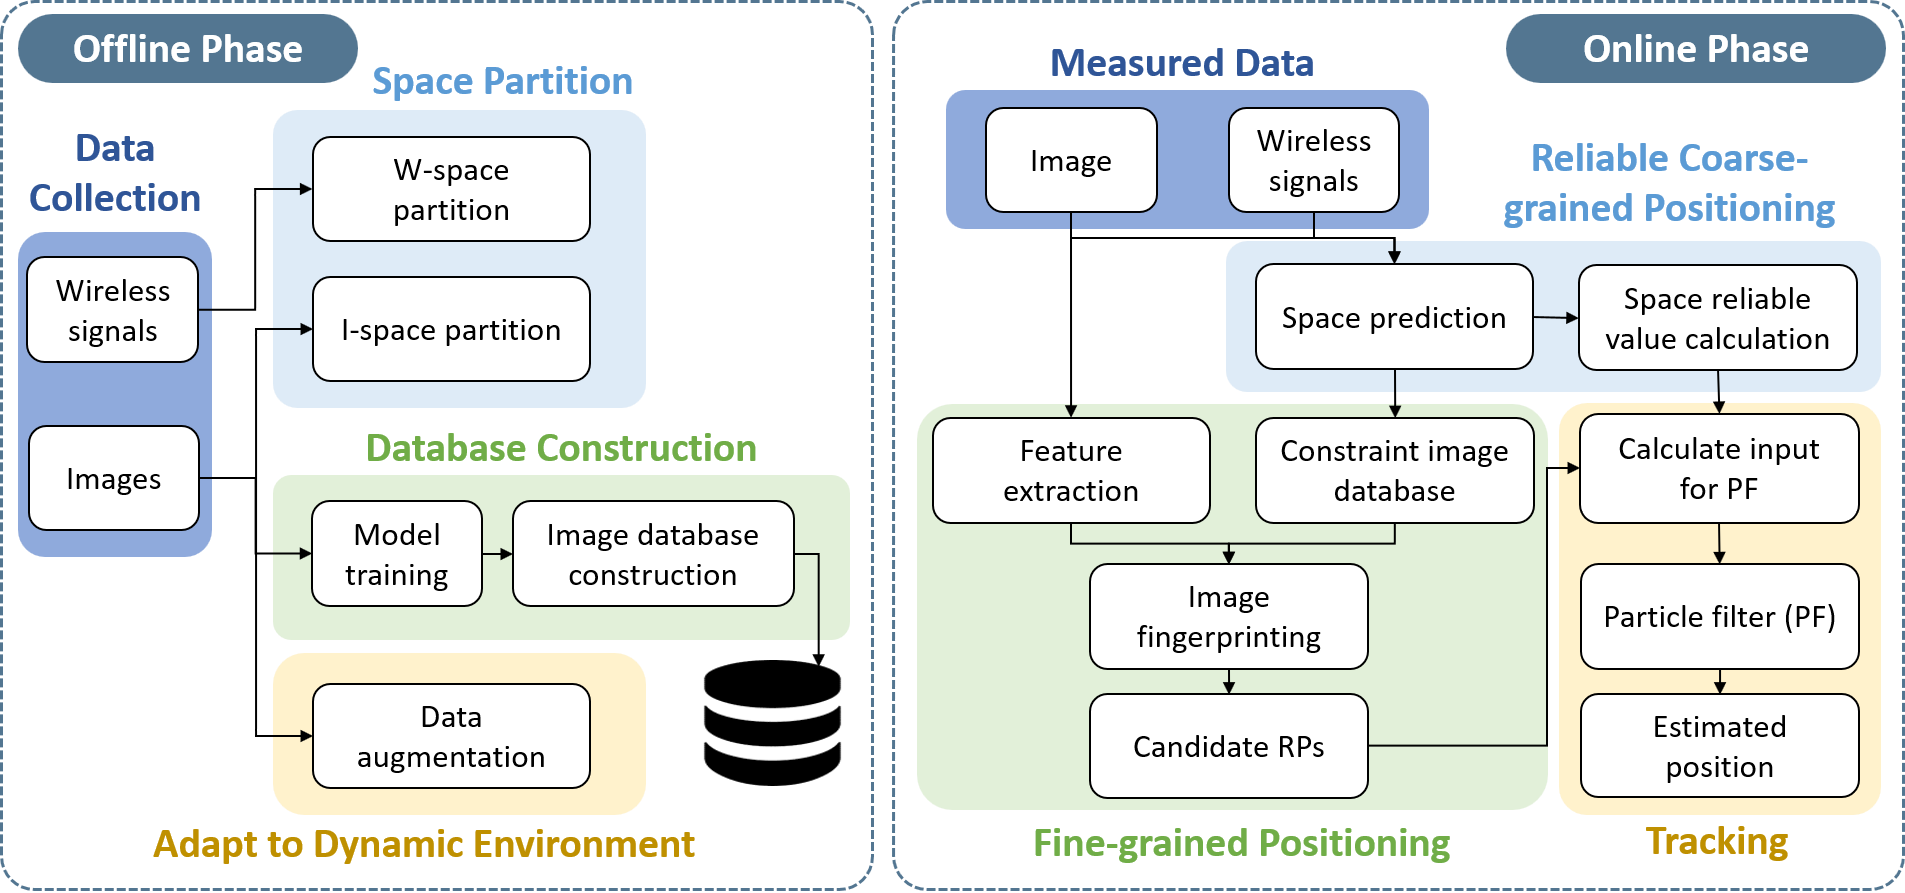
\includegraphics[width=\columnwidth]{images/chap3/overall_sys_architecture.png}
    \caption{Overall system architecture.}
    \label{Fig:overall_system_architecture}
    \end{center}
\end{figure}
In the offline phase, the first step is to collect wireless signals and images in the indoor environment. Next, space partition utilizes two types of data to divide the indoor space into multiple regions. These regions can be used to predict the approximate user location in online phase. Then, we train a model to extract image features and build an image database for fingerprinting. Lastly, to adapt the model to dynamic indoor environments, we propose a data augmentation method to enhance performance of the model. The online phase adopts a hierarchical structure and is divided into two stages, coarse-grained positioning and fine-grained positioning. We first use wireless signals and images to predict the approximate space where the user is located. Based on an algorithm, we assign reliable values to each space, making the results more trustworthy. Then, within the predicted space, we perform precise localization using image fingerprinting techniques. Finally, the particle filter algorithm is utilized to track the user's position and improve the accuracy of the localization results.


% ---------------- section 3.1 ----------------
\section{Offline Phase}
\paragraph{}
Below, we will introduce the offline phase, which consists of five subsections: data collection, space partition, model training, image database construction, and data augmentation.

\subsection{Data Collection}
\subsubsection{Wireless Signals}
\paragraph{}
For wireless training data, we collect RSSI measurements at each reference point for a fixed period of time. We denote the $j$-th wireless sample at reference point $i$ as $W_{i,j}=\left[ r_{i,j}^1,r_{i,j}^2,\ldots,r_{i,j}^{|B|} \right]$, where $B$ is the set of wireless beacons deployed in the environment and $r_{i,j}^b$, $b=1,2,\dots,|B|$ is the $j$-th average RSSI measurement of beacon $b$ at the reference point $i$. Then we use the Min-Max normalization formula (\ref{Eq:min_max_normalization}) to normalize the RSSI measurements. $r_{max}^b$ and $r_{min}^b$ are the maximum and minimum RSSI value collected from beacon $b$.
\begin{equation}
    \label{Eq:min_max_normalization}
    \hat{r_{i,j}^b}=\frac{r_{i,j}^b-r_{min}^b}{r_{max}^b-r_{min}^b}
\end{equation}

\subsubsection{Image Data}
\paragraph{}
For image training data, we record a 360-degree video while rotating at each training location. We represent the video collected at reference point $i$ as $I_i=\{f_i^1,f_i^2,\dots\}$ where $f_i^j$ refers to $j$-th frame of video at reference point $i$.
\subsection{Space Partition}
\paragraph{}
In order to achieve coarse-grained positioning during the online phase, we divide the indoor space into multiple areas. Due to the different characteristics of the data, different methods are used for space partition for wireless signals and images, referred to as W-space partition and I-space partition, respectively.
\subsubsection{W-space Partition}
\paragraph{}
To partition the space using wireless signal information, we use the improved K-means algorithm \cite{zhang2020received} to perform W-space partition. In other words, we cluster the reference points in the map. The reference points are allowed to be included in more than one clusters, i.e., the obtained clusters can overlap with one another.
\paragraph{}
Initially, we use the standard K-means algorithm to assign all collected wireless signals to $K$ clusters $C=\{c_1,c_2,\dots,c_K\}$. Meanwhile, we find the clusters' centers $\mu_C=\{\mu_C(1),\mu_C(2),\dots,\mu_C(K)\}$ and the maximum distance between the data point and its center in each cluster $d_{train}^{max}=\{d_{train}^{max}(1),d_{train}^{max}(2),\dots,d_{train}^{max}(K)\}$.
\paragraph{}
Next, we determine which W-spaces a reference point belongs to by calculating the ratio of the number of RSSI samples from this reference point in each cluster to the total number of RSSI samples collected at this reference point. Suppose that in cluster $c_k$, there are $num_k^i$ samples from reference point $i$. Then the ratio $num_k^i/m_i$ is calculated, where $m_i$ denotes the number of samples collected at reference point $i$. If the ratio greater than a threshold $p$, we have that cluster $c_k$ contains significant amount of samples from reference point $i$, so reference point $i$ is assigned to W-space $k$. The example result of W-space partition ($K=4$) is show in figure \ref{Fig:wspace_partition}.

\subsubsection{I-space Partition}
\paragraph{}
Partitioning the space based on images is a relatively easy task. We can simply use human visual perception to divide the indoor space into different areas. According to our experimental environment, the indoor space is divided into four areas, namely: server area, seating area, public aisle and public area. 
\paragraph{}
The server area is characterized by computer screens, mainframes, and similar equipment. It typically does not contain chairs or personal belongings, resulting in relatively minimal changes in the environment. On the other hand, the seating area is more diverse, with each seat potentially having different objects like coffee mugs, books, and other personal items. These objects are prone to frequent changes in their positions. The public aisle and public area are relatively open spaces, with the distinction being that the public area includes conference tables. The partition result is shown in Figure \ref{Fig:ispace_partition}.
\begin{figure}[h]
    \centering
    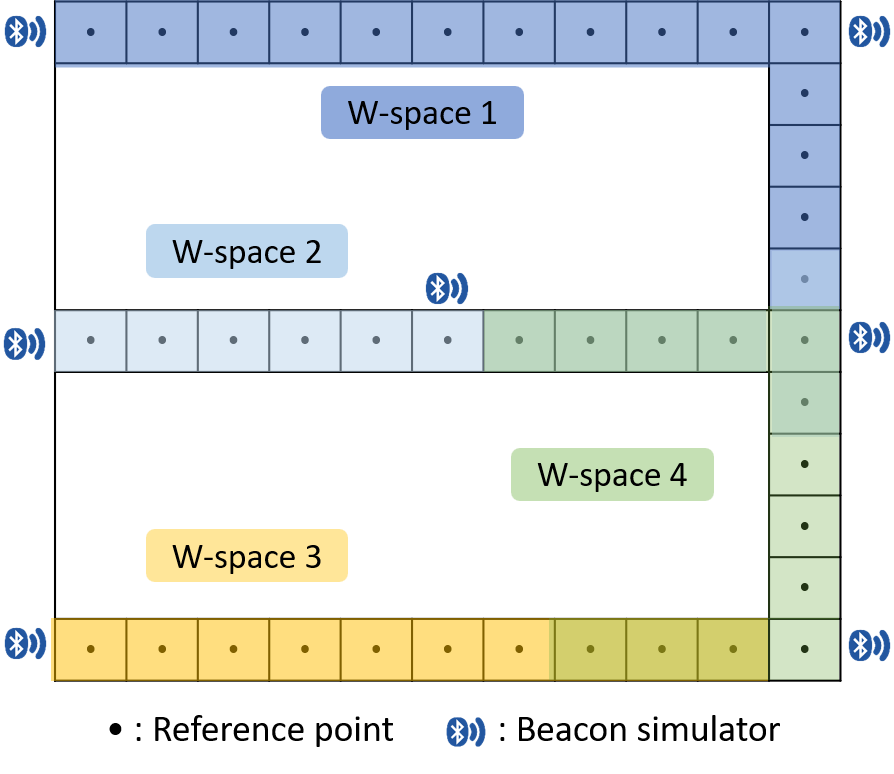
\includegraphics[width=0.5\columnwidth]{images/chap3/wspace_partition.png}
    \caption{Result of W-space partition, $K=4$.}
    \label{Fig:wspace_partition}
\end{figure}
\begin{figure}[h]
    \centering
    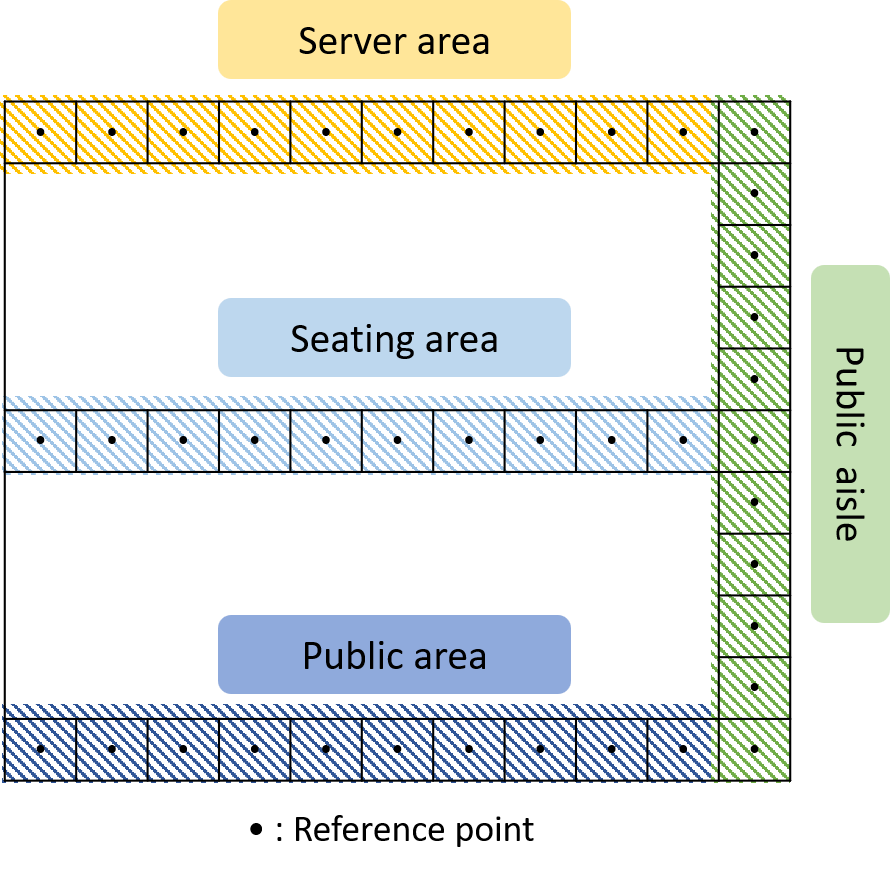
\includegraphics[width=0.5\columnwidth]{images/chap3/ispace_partition.png}
    \caption{Result of I-space partition.}
    \label{Fig:ispace_partition}
\end{figure}


\subsection{Model Training}
\paragraph{}
Due to the mature development of machine learning in the field of image processing, we trained a Convolutional Neural Network (CNN) to process image data. The proposed multi-level label CNN model architecture is shown in Figure \ref{Fig:cnn_model}. To enable the model to run easily on mobile devices, we chose a lightweight backbone, MobileNetV3 small. Two classifiers are connected after the fully connected layer, one for I-space classification and the other for RP classification. The label of the I-space classifier is the result of I-space partition, which provides the model with coarse-grained environmental information. In addition, during the online phase, the predicted I-space by the model is used as the coarse-grained positioning result of the image. On the other hand, the RP classifier provides the model with fine-grained environmental features. Through the I-space and RP classifiers, the model can learn both macro and micro image features.
\paragraph{}
\begin{figure}[h]
    \centering
    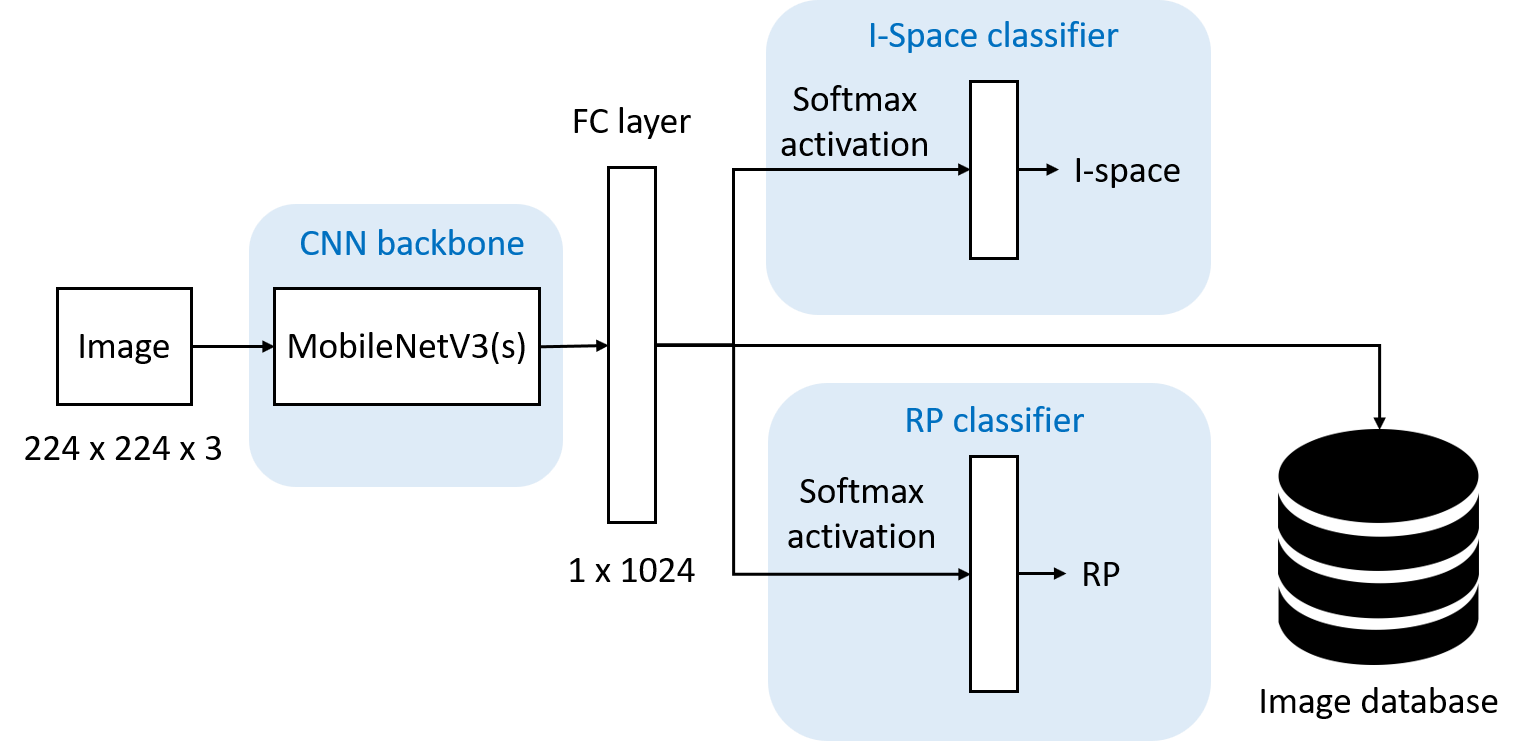
\includegraphics[width=0.8\columnwidth]{images/chap3/cnn_model.png}
    \caption{Multi-level label CNN model architecture.}
    \label{Fig:cnn_model}
\end{figure}
To enable the model to be quickly trained in different environments, we fine-tune the CNN model with pre-trained weights on ImageNet 1k, so the training process can be completed in a short period of time. We set the learning rate to 0.001 and use Adam as the optimizer. The loss of I-space classification and reference point classification are calculated by cross entropy, then sum up to get the total loss. The loss function is shown below. $N$ is the number of I-spaces and $|RP|$ is the number of reference points. $t_{is}^c$ is the truth label and $p_{is}^c$ is the Softmax probability for the class $c$, for I-space. Similarly, $t_{rp}^c$ is the truth label and $p_{rp}^c$ is the Softmax probability for the class $c$, for reference point.
\begin{align}
    \label{Eq:loss_functions}
    L_{ispace}&=-\sum_{c=1}^N\ t_{is}^c\ \log(p_{is}^c) \\
    L_{rp}&=-\sum_{c=1}^{|RP|}\ t_{rp}^c\ \log(p_{rp}^c) \\
    L_{total}&=L_{ispace}+L_{rp}
\end{align}


\subsection{Image Database Construction}
\paragraph{}
We take the output of the fully connected layer in the CNN model as the image feature (vector of size $1\times1024$). For the $j$-th frame image collected at the reference point $i$, $f_i^j$, its image feature is denoted as $\hat{f_i^j}$. The set of image features from reference point $i$ is denoted as $\hat{I_i}$.
\paragraph{}
To reduce the fingerprinting time during the online phase, we used the ball tree algorithm to construct a tree-like structure for the database. Compared to the traditional KNN algorithm, the ball tree can improve search time from $O(n)$ to $O(\log n)$ \cite{bhatia2010survey}. We construct the trees for each W-space and I-space. For instance, W-space $k$ includes reference point $a$ and $b$, we then use the corresponding image features from reference point $a$ and $b$ to construct a ball tree $T_w(k)$. The same approach is applied to each W-space and I-space. As a result, we can get the image database:
\begin{equation}
    \label{Eq:DB_image}
    DB_{image}=\{T_w,T_i\}=\{T_w(1),\dots,T_w(k),T_i(1),\dots,T_i(N)\}
\end{equation}
 
\subsection{Data Augmentation}
\paragraph{}
Based on observations of the indoor environment, we have noticed that objects that are easily movable contribute to the dynamic nature of the indoor scene. To prevent the multi-level label CNN model from being affected by changes in objects in the indoor environment, we occluded the objects in photos to achieve data augmentation and enable the model to perform well in dynamic indoor environments. We use the YOLOv7 \cite{wang2023yolov7} package to complete the masking task. YOLOv7 can do instance segmentation in the image and generate corresponding labels. Using these label information, we can easily obtain a new image with the objects occluded.
\paragraph{}
For an image $f_i^j$, the first step is to detect the object categories and their polygon labels in the image using YOLOv7. Assuming that $M$ objects are detected in the image, the category and polygon label of the $m^{th}$ object can be represented as $obj_{cat}^m$ and $obj_{pg}^m$. Additionally, we predefine the masking rate and portable rate beforehand. The portable rate is a value defined based on the mobility of an object. Different portable rates are assigned to different object categories. Objects that are easy to move, such as mugs or backpacks, are given a higher portable rate, while objects that are less likely to be moved, such as dining tables or refrigerators, are given a lower portable rate. The portable rate of category $c$ is represented as $pr_c\in(0,1)$. The masking rate represents the proportion of candidate obstructed objects in the image and is denoted as $mr$. The higher the masking rate, the more objects are likely to be obstructed in the image. 
\paragraph{}
Algorithm \ref{Algo:obj_masking} shows the pseudo code of the object masking algorithm. Initially, the masking rate $mr$ is used to determine the candidate occlusion objects. Then, for each candidate object, the portable rate of its category is used to decide whether it should be occluded. If the object is confirmed to be occluded, its polygon label is converted to a pixel label, and then each pixel is filled with a value ranging from $0$ to $255$ to complete the occlusion process. Finally, we get the new image $\widetilde{f_i^j}$. Examples of original and masked images are shown below:

% ========== Algorithm ========== %
\begin{algorithm}[H]
    \SetAlgoLined
    \DontPrintSemicolon
    \caption{Object Masking}
    \label{Algo:obj_masking}
    \BlankLine
    \KwIn {$f_i^j$}
    \KwOut {$\widetilde{f_i^j}$}
    \BlankLine
    copy $f_i^j$ to $\widetilde{f_i^j}$ \;
    $Obj=YOLOv7(\widetilde{f_i^j})$ \tcp*[l]{Object detection.}
    $Obj=$ select candidate objects in $Obj$ by masking rate $mr$ \;
    $M=|Obj|$ \tcp*[l]{Number of candidate objects.}
    \For{$m=1\ to\ M$ }{
        $c=obj_{cat}^m$ \tcp*[l]{Category of object.}
        $p=Random(0,1)$ \;
        \uIf{$p\leq pr_c$}{ \tcp*[l]{Mask the object.}
            convert $obj_{pg}^m$ to $obj_{px}^m$ \tcp*[l]{Polygon label to pixel label.}
            \For{$pixel$\ in\ $obj_{px}^m$}{
                $pixel$ in $\widetilde{f_i^j}=Random(0,255)$
            }
        }
    }
    \Return $\widetilde{f_i^j}$
\end{algorithm}

\begin{figure}[htbp]
    \centering
    \subfloat[Original image]{
        \begin{minipage}[t]{0.45\columnwidth}
            \centering
            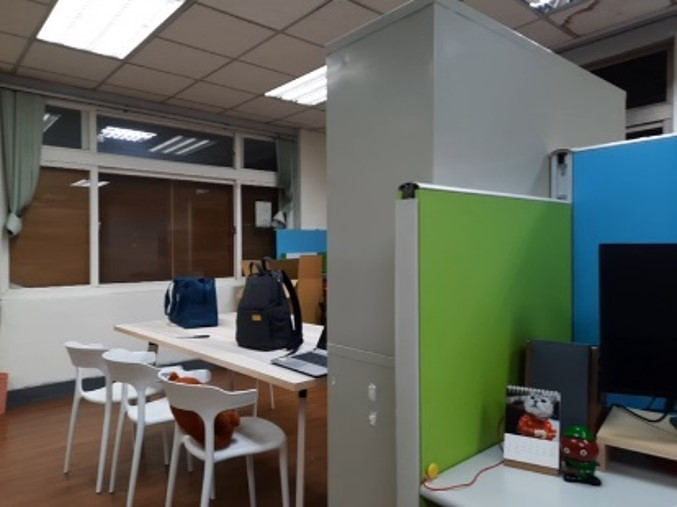
\includegraphics[width=0.9\textwidth]{images/chap4/no_mask.jpg}
        \end{minipage}
    }
    \subfloat[Masked image]{
        \begin{minipage}[t]{0.45\columnwidth}
            \centering
            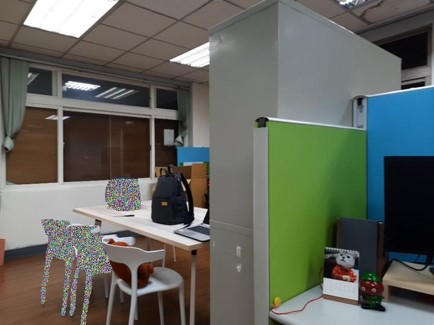
\includegraphics[width=0.9\textwidth]{images/chap3/mask.jpg}
        \end{minipage}
    }
    \label{Fig:maksing_result}
    \caption{The image before and after masking.}
\end{figure}

% ---------------- section 3.2 ----------------
\section{Online phase}
\paragraph{}
To achieve more accurate localization results, we adopt a hierarchical architecture with two processes, namely reliable coarse-grained and fine-grained positioning. In reliable coarse-grained positioning, we utilize wireless signal $w$ and image $i$ to predict the W-space and I-space. Then, based on an intuitive and non-complex algorithm, we assign a reliable value to each space, aiming to make the results more trustworthy. Next, we extract feature $\hat{i}$ from the image using multi-level label CNN model for fine-grained positioning, which is a fingerprinting process. In the fingerprinting process, we utilize the results of coarse-grained localization to constrain the range of the database and search the top $k$ samples as candidate reference points. Finally, we calculate the input for particle filter and track the user's position. 
\subsection{Coarse-grained Positioning}
\paragraph{}
In the coarse-grained positioning, wireless signal and image are used to predict the W-space and I-space, respectively. The algorithm is then applied to assign reliable value to each space, which improves the reliability of the localization results in this stage.

\subsubsection{Space Prediction}
\paragraph{}
For W-space prediction, firstly, normalize the measured wireless signal $w$ to obtain its normalized value $\hat{w}$ through formula (\ref{Eq:min_max_normalization}). Then, find the minimum Euclidean distance between all the centers in $\mu_C$ and $\hat{w}$ in order to predict the W-space, denoted as $space_w$. The calculation formula is shown in formula (\ref{Eq:find_closest_center}). Meanwhile, we also save the minimum distance as $d$. 
\begin{equation}
    \label{Eq:find_closest_center}
    space_w=\min_{k=1,2,\dots,K} \left\| \mu_C(k)-\hat{w} \right\|_2
\end{equation}
\paragraph{}
For the I-space prediction, since it is one of the outputs of the multi-level lable CNN model (Figure \ref{Fig:cnn_model}), it can be directly predicted by the model and denoted as $space_i$.

\subsubsection{Space Reliable Value Calculation}
\paragraph{}
After obtaining $space_w$ and $space_i$, we can calculate the reliable values of two spaces. The purpose is to give each space different reliable value according to the situation, so that the coarse-grained result can be more reliable. Algorithm \ref{Algo:CV} shows the pseudo code of space reliable value calculation.
\paragraph{}
First, based on $space_w$ and $space_i$, we find the set of reference points within the two spaces, which are $RP_w$ and $RP_i$. Next, based on the intersection $RP_w\cap RP_i$, we define the reliable value $r_w$ and $r_i$ of W-space and I-space. If the intersection of the two collections is not empty, it means that the predicted spaces by wireless signal and image are close to each other. Thus, we give the same reliable value, which is $0.5$, to the two spaces. On the other hand, if the intersection of the two collections is empty, it means that only one of the wireless signal or image predictions is trustworthy. In this case, we will check whether the received wireless signal $w$ is stable. If the distance between $\hat{w}$ and the center of its corresponding cluster $space_w$ is smaller than the maximum distance between all data points in $space_w$ and its center, then $w$ is considered an inlier and thus $w$ is stable. On the other hand, if $w$ is an outlier, then $w$ is considered unstable. Since the $d_{train}^{max}$ already records the maximum distances between data points and centers within each cluster, we can compare the value of $d$ and $d_{train}^{max}(space_w)$ directly.
\paragraph{}
If $d$ is less than or equal to $d_{train}^{max}(space_w)$, it means that the wireless signal is stable, and we can trust the result of W-space. Therefore, we give a reliable value to $r_w$ that is higher than $r_i$. Conversely, if $d$ is greater than $d_{train}^{max}(space_w)$, it means that the wireless signal is unstable, and we should trust the result of I-space instead. In this case, we give a higher reliable value to $r_i$ than $r_w$.

% ========== Algorithm ========== %
\begin{algorithm}[H]
    \SetAlgoLined
    \DontPrintSemicolon
    \caption{Space Reliable Value Calculation}
    \label{Algo:CV}
    \BlankLine
    \KwIn {$space_w,space_i,d,d_{train}^{max}$}
    \KwOut {$r_w,r_i$}
    \BlankLine
    $r_w=r_i=0$ \tcp*[l]{Initialization.}
    $RP_w=a\ set\ of\ RPs\ in\ space_w$ \;
    $RP_i=a\ set\ of\ RPs\ in\ space_i$ \;
    \eIf{$RP_w$ intersects $RP_i$ is not empty}{
        $r_w=0.5$ \;
        $r_i=0.5$ \;
    }{
        $l=d_{train}^{max}(space_w)$ \;
        \eIf{$d\leq l$}{
            assign $r_w$ value larger than $r_i$ \tcp*[l]{$r_w+r_i$ must be $1$}
        }{
            assign $r_i$ value larger than $r_w$ \tcp*[l]{$r_w+r_i$ must be $1$}
        } 
    }
    \Return $r_w,r_i$
\end{algorithm}


\subsection{Fine-grained Positioning}
\paragraph{}
During the fine-grained positioning, we find some candidate reference points from the image database $DB_{image}$ through fingerprinting. To save matching time, we do not compare every sample in the image database, but instead select a portion of  database for fingerprinting based on the coarse-grained positioning results.
\paragraph{}
To begin with, we extract the image feature $\hat{i}$ from the measured image data $i$. Then, based on coarse-grained positioning results $space_w$ and $space_i$, we constraint the range of image database. In other words, we find the corresponding trees in $DB_{image}$, which are $T_w(space_w)$ and $T_i(space_i)$, respectively. We search for the top $k$ samples in two trees, and record the reference point of the top $k$ samples to obtain candidate reference points. Since the data within the tree corresponds to the RP samples belonging to that space, we can ensure the selected candidate reference points are within the range of the space, achieving a hierarchical localization. Algorithm \ref{Algo:fine_grained_positioning} shows the fine-grained positioning process.
\paragraph{}
% ========== Algorithm ========== %
\begin{algorithm}[H]
    \SetAlgoLined
    \DontPrintSemicolon
    \caption{Fine-grained Positioning}
    \label{Algo:fine_grained_positioning}
    \BlankLine
    \KwIn {$space_w,\ space_i,\ i,\ DB_{image}$}
    \KwOut {$RP_{cand}$}
    \BlankLine
    $RP_{cand}=\left[ \ \right]$ \tcp*[l]{Initialization.}
    extract image feature $\hat{i}$ from $i$ \tcp*[l]{By multi-level label CNN model.}
    $T=\{\ T_w(space_w),\ T_i(space_i)\ \}$ \tcp*[l]{Constraint the $DB_{image}$.}
    \For{tree in\ $T$}{
        search top $k$ samples in tree \tcp*[l]{Fingerprinting.}
        add reference point of samples to $RP_{cand}$
    }
    \Return $RP_{cand}$
\end{algorithm}

\subsection{Tracking}
\paragraph{}
To achieve higher positioning accuracy, we use the particle filter at the end of the online phase to track position of the user. The particle filter operates in a recursive manner, updating the state estimate as new input of particle filter become available. In our particle filter, we propose a novel input called ``RP scor'' to update the weights of particles.

\subsubsection{RP Score Calculation}
\paragraph{}
After the coarse-grained positioning, we can get space reliable value $r_w$ and $r_i$. We utilize the space reliable value and candidate reference points $RP_{cand}$ obtained from fine-grained positioning to calculate scores for each RP, which serve as the basis for updating the particle filter's particle weights.
\paragraph{}
For each candidate RP, we start by conducting a vote, which involves counting the number of times each RP appears. For the $i$-th RP, its vote count is recorded as $VT^i$. Next, we calculate the reliable value for each RP based on the space it belongs to. If the $i$-th RP is present in both W-space and I-space, its reliable value is calculated as $RV^i=r_w+r_i$. If the RP belongs to only one of the spaces, its reliable value is either $r_w$ or $r_i$, depending on the space it belongs to. The formula is shown below:
\begin{equation}
    \label{Eq:RP_RV}
    RV^i=\begin{cases}
        r_w+r_i, &\text{RP in both $RP_w$ and $RP_i$}\\
        r_w, &\text{RP only in $RP_w$}\\
        r_i, &\text{RP only in $RP_i$}
    \end{cases} \\  
\end{equation}
\paragraph{}
Finally, the score for the $i$-th RP is calculated by multiplying its vote count ($VT^i$) with its reliable value ($RV^i$).
\begin{equation}
    \label{Eq:RP_score}
    score^i=VT^i\times RV^i
\end{equation}
\begin{equation}
    \label{Eq:RP_score_normalize}
    \hat{score^i}=\frac{score^i}{\sum_j{score^j}}
\end{equation}

\subsubsection{Particle Filter}
\paragraph{}
Figure \ref{Fig:pf} shows the flow of particle filtering. The process of the particle filter is as follows:
\paragraph{}
Step 1: Initialization. At the every beginning, the particles are evenly spread across the map, and each particle is assigned the same weight. This ensures that the initial set of particles covers the entire area of interest uniformly and does not favor any specific location.
\paragraph{}
Step 2: Update. We can update the $j$-th particle weights using formula (\ref{Eq:update_weight}). Here, $d^i$ represents the distance between the particle and the $i$-th reference point. From the formula, we can understand that the closer the particle is to the reference point and the higher the score of reference point, the particle will receive a higher weight.
\begin{equation}
    \label{Eq:update_weight}
    w_j^{'}=\sum_{i\in RP_{cand}}{w_j\times {e^{-0.5\times d^2}} \times \hat{score^i}}
\end{equation}
\paragraph{}
Step 3: Resample. After updating, the weights will be normalized and particles are resampled according to the weights. The larger the weight of a particle, the more likely it is to be sampled. After resampling, the distribution of particles on the map changes, forming new states, and each particle is given the same weight again.
\paragraph{}
Step 4: Prediction. After resampling, we can use the new particle states to predict the user's location. By multiplying the weight of each particle by its coordinate position, we can calculate the weighted position.
\begin{align}
    \label{Eq:position_calculation}
    x&=\sum_j{w_j^{'}\times x_j} \\
    y&=\sum_j{w_j^{'}\times y_j}
\end{align}
\paragraph{}
\begin{figure}[h]
    \centering
    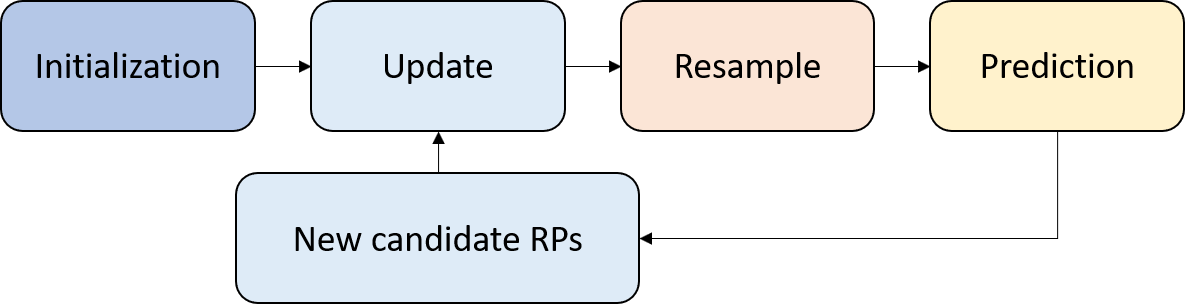
\includegraphics[width=0.8\columnwidth]{images/chap3/pf.png}
    \caption{Particle filter.}
    \label{Fig:pf}
\end{figure}
% ---------------- section 3.3 ----------------
\section{Expansion for the Multi-device System}
\paragraph{}
Our system is highly flexible and can easily be expanded to achieve multi-device positioning. The online process for a multi-device system is illustrated in the figure \ref{Fig:multi_device}. For the $n$-th device, it predicts its own W-space and I-space, and calculates the space reliability value $r_w^n$ and $r_i^n$. Then, through fine-grained positioning process, the device can obtain its candidate reference points $RP_{cand}^n$.
\paragraph{}
Next, we integrate the information from multiple devices during the RP score calculation. During the voting process, we collectively vote on all candidate reference points from all devices and calculate the number of votes for each candidate reference point. When calculating the reliable value for the $i$-th candidate reference point, we check if the reference point is included in the predicted W-space and I-space of each device and sum up the corresponding space reliability values. The formula is as follows:
\begin{equation}
    \label{Eq:multi_device}
    RV^i=\sum{r_{space}^{device}} \text{, if RP in space of device.}
\end{equation}
\paragraph{}
Finally, based on equations (\ref{Eq:RP_score}) and (\ref{Eq:RP_score_normalize}), we can obtain the RP score. By doing so, we can expand our system into a multi-device indoor positioning system through simple calculations.
\paragraph{}
\begin{figure}[h]
    \centering
    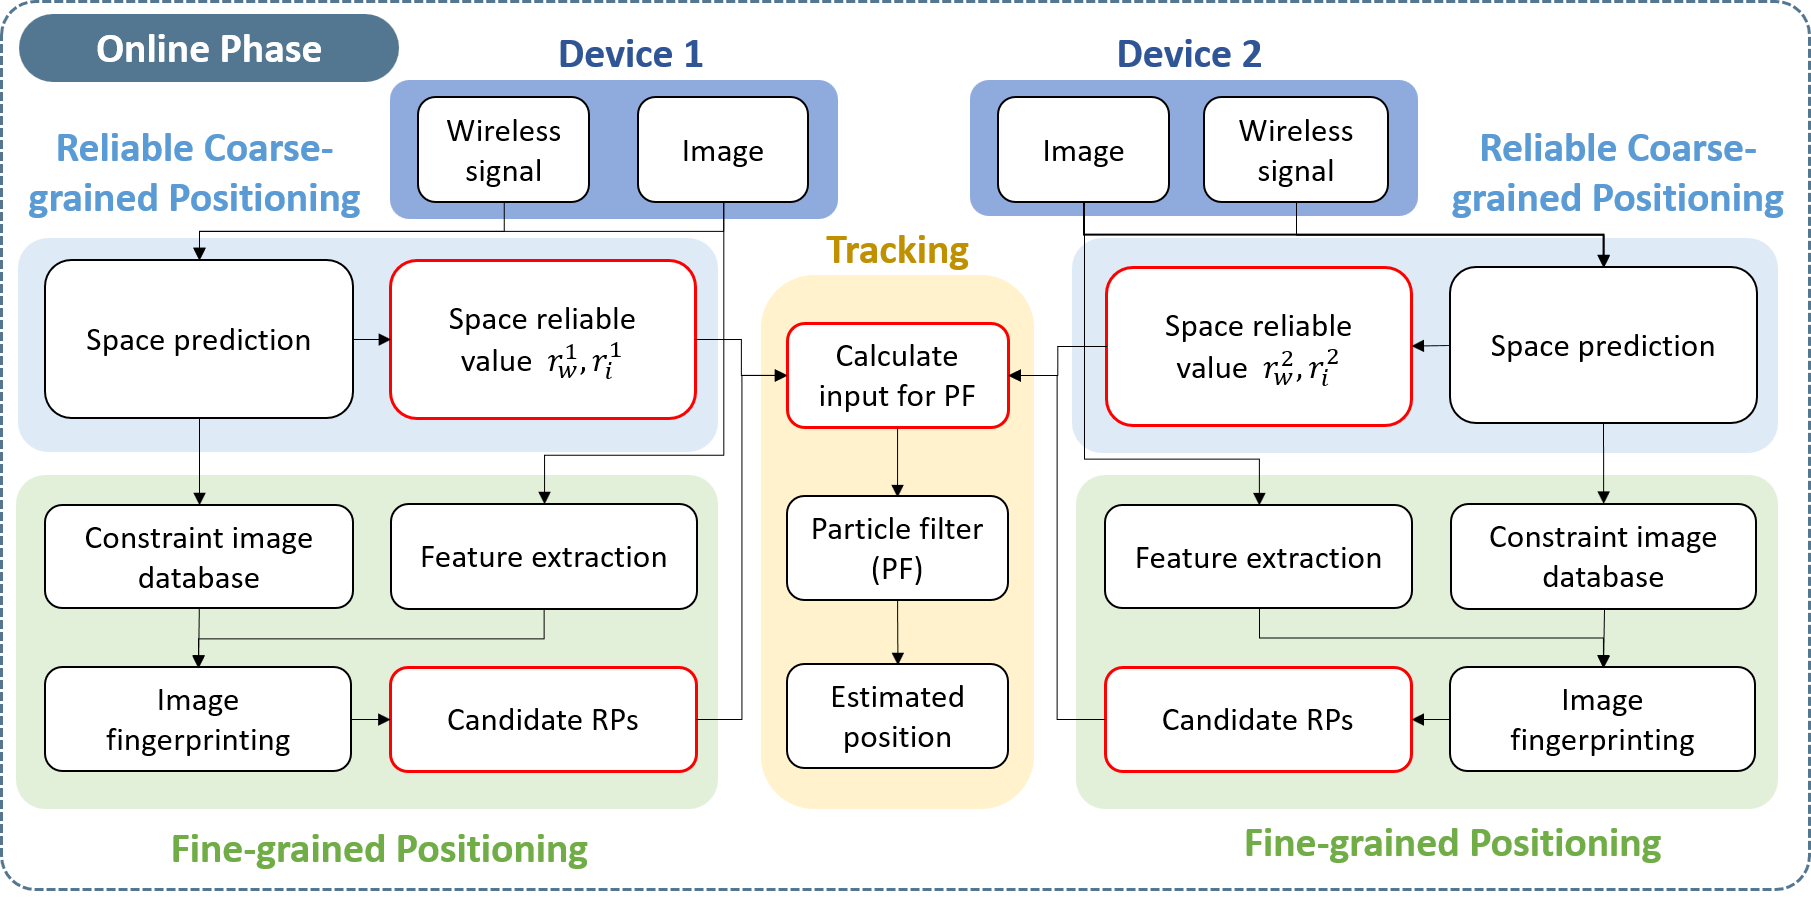
\includegraphics[width=\columnwidth]{images/chap3/multi_device.png}
    \caption{Online phase process for multi-device positioning.}
    \label{Fig:multi_device}
\end{figure}



% ---------------- chapter 4 ----------------
\chapter{Experimental Setup}
\section{Experimental Environment}
\paragraph{}
An office room 92589 located in the Electrical Engineering (EE) Department of National Cheng Kung University (NCKU), Tainan, Taiwan is our experimental environment, as shown in figure \ref{Fig:room_92589}. As can be seen from the experiment environment, there are some common objects such as chairs, computer monitors, and keyboards, as well as personal items on the desk and shelves. Overall, this experimental environment represents a real office situation.
\begin{figure}[htbp]
    \begin{center}
    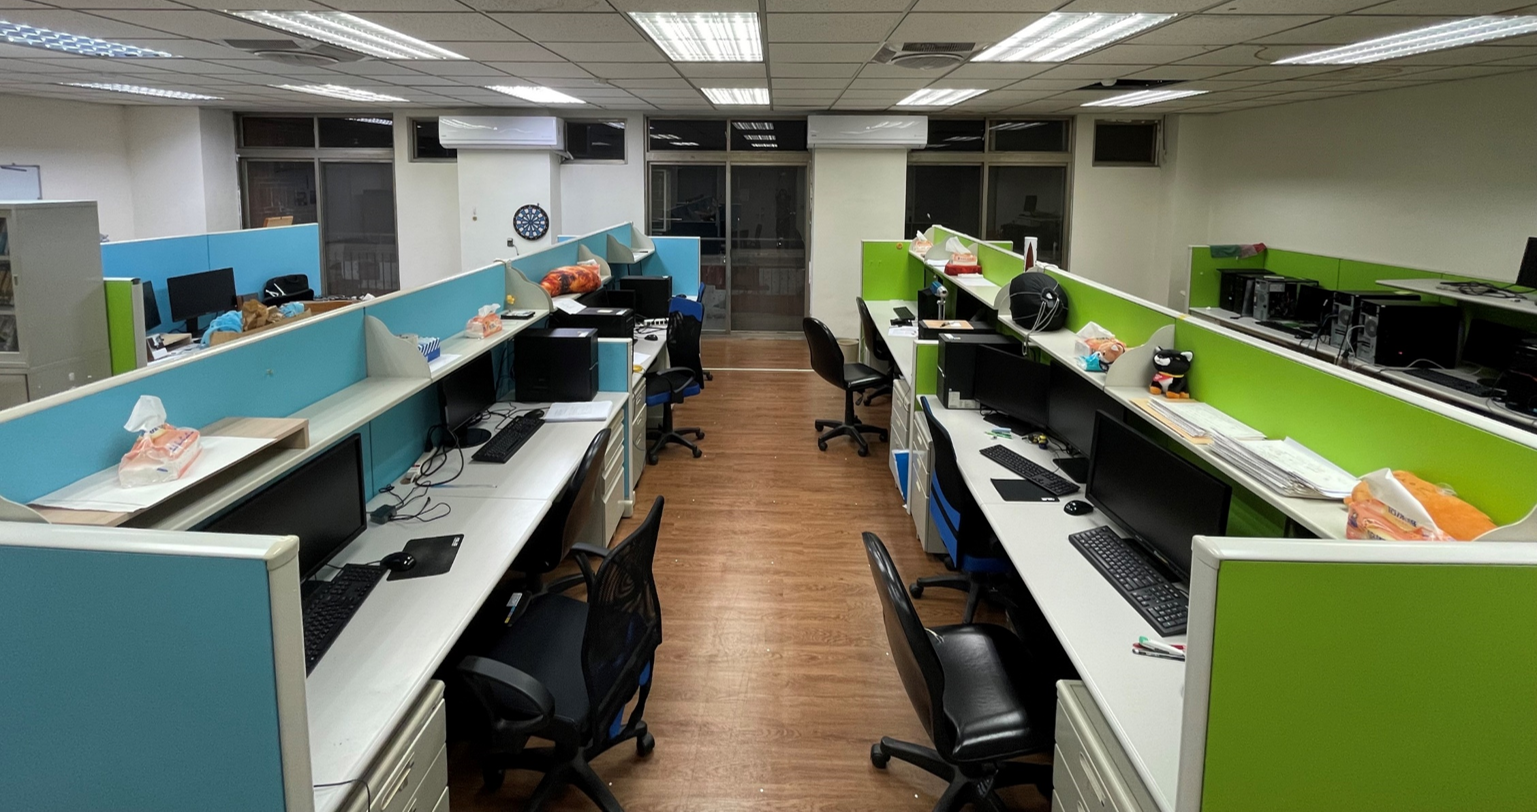
\includegraphics[width=\columnwidth]{images/chap4/room_92589.png}
    \caption{Experimental environment.}
    \label{Fig:room_92589}
    \end{center}
\end{figure}

\paragraph{}
Figure \ref{Fig:floor_plan} is a floor plan. In the floor plan, we conduct the experiment within the area of the M-shaped corridor, which has $41$ reference points, with each reference point having a length and width of $0.6$ meters. The figure also shows the deployment of the Bluetooth Low Energy (BLE) beacons, with a total of $7$ beacons, each placed $1.2$ meter off the ground.
\begin{figure}[htbp]
    \begin{center}
    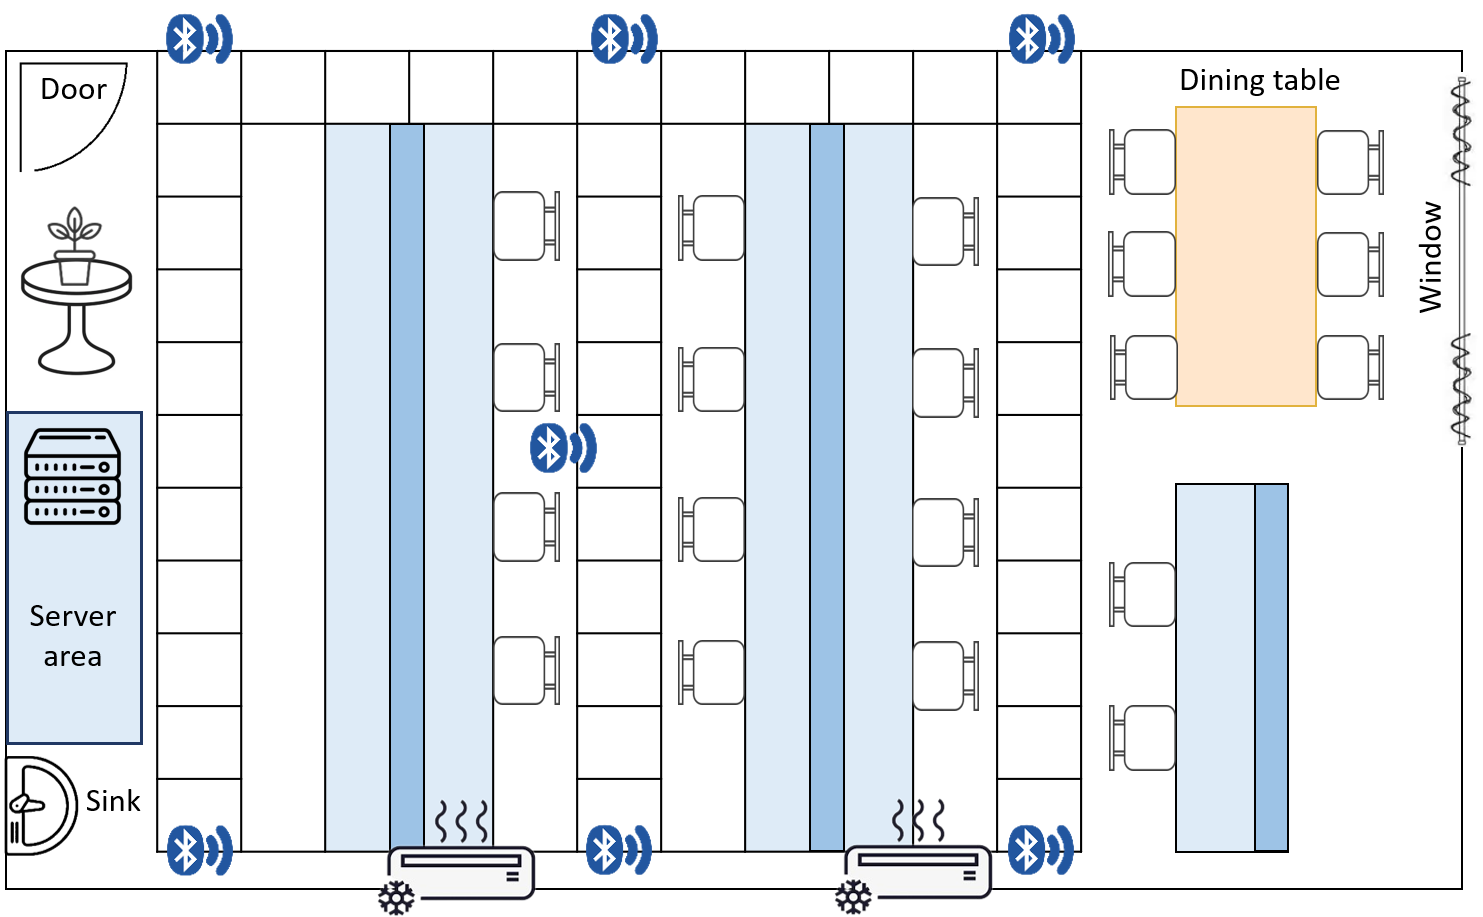
\includegraphics[width=\columnwidth]{images/chap4/floor_plan.png}
    \caption{Floor plan of the indoor environment.}
    \label{Fig:floor_plan}
    \end{center}
\end{figure}

\section{Experimental Scenarios}
\paragraph{}
In the experiment, we simulate the situation where the user holds a phone in front of their chest and moves around. The phone directly receives wireless signals from the beacons, and the image represents the scene in front of the user, as shown in the figure \ref{Fig:simulate}. We design three scenarios to simulate the different mobility of the user, namely Stationary, Scripted Walk and Free Walk.
\begin{itemize}
    \item Stationary: A stationary fixed point. We selected several locations in the indoor environment and remained stationary at each location to simulate the user stays at a fixed point for a period of time. The location map of the stationary scenario is shown in Fig.
    \item Scripted Walk: A regular walking path. In this scenario, we simulate the user walking regularly in the environment, mostly in the same direction, as shown in the figure.
    \item Free Walk: The opposite of a scripted walk, this scenario simulates the user moving freely and unpredictably, possibly wandering back and forth in one region, or suddenly turning back halfway through the walk, etc.
\end{itemize}
\begin{figure}
    \centering
    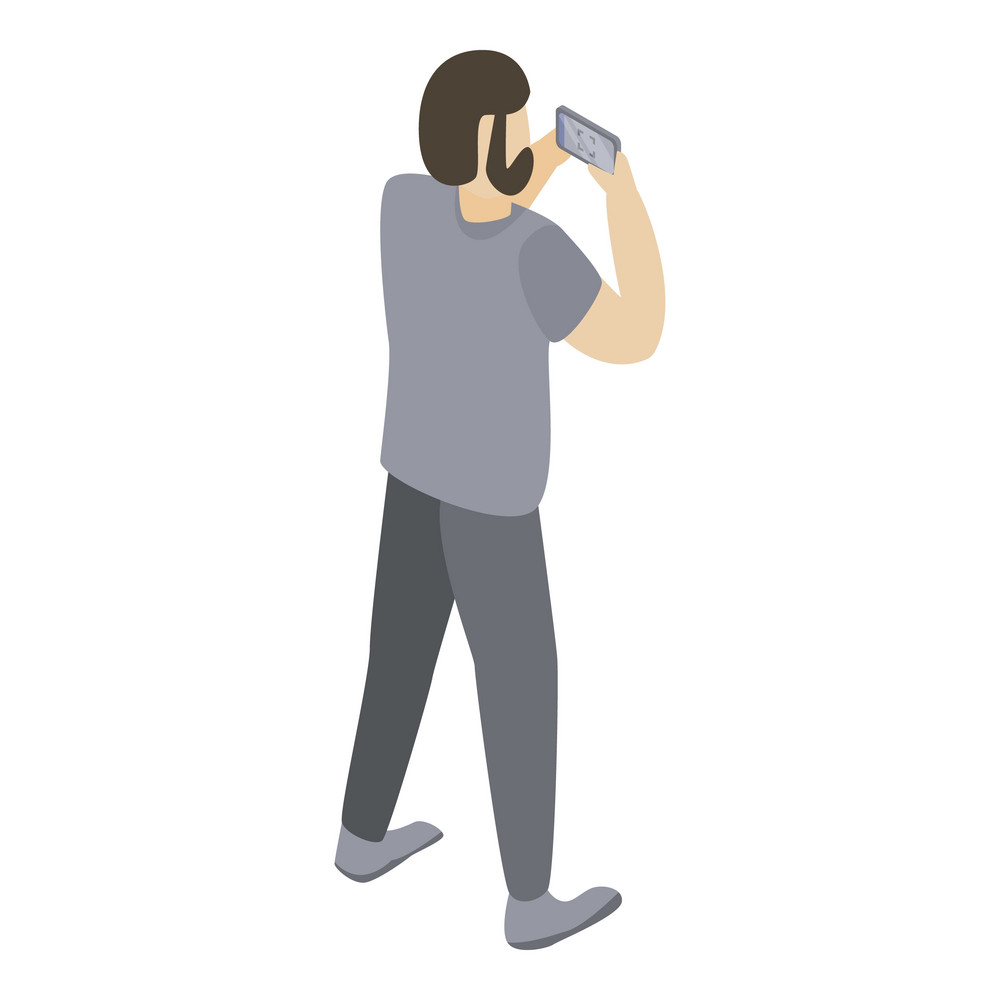
\includegraphics[width=0.3\columnwidth]{images/chap4/simulate.png}
    \caption{Illustration of usage scenario.}
    \label{Fig:simulate}
\end{figure}

\paragraph{}
\begin{figure}[htbp]
    \centering
    \subfloat[Positions of Stationary]{
        \begin{minipage}[t]{0.48\columnwidth}
            \centering
            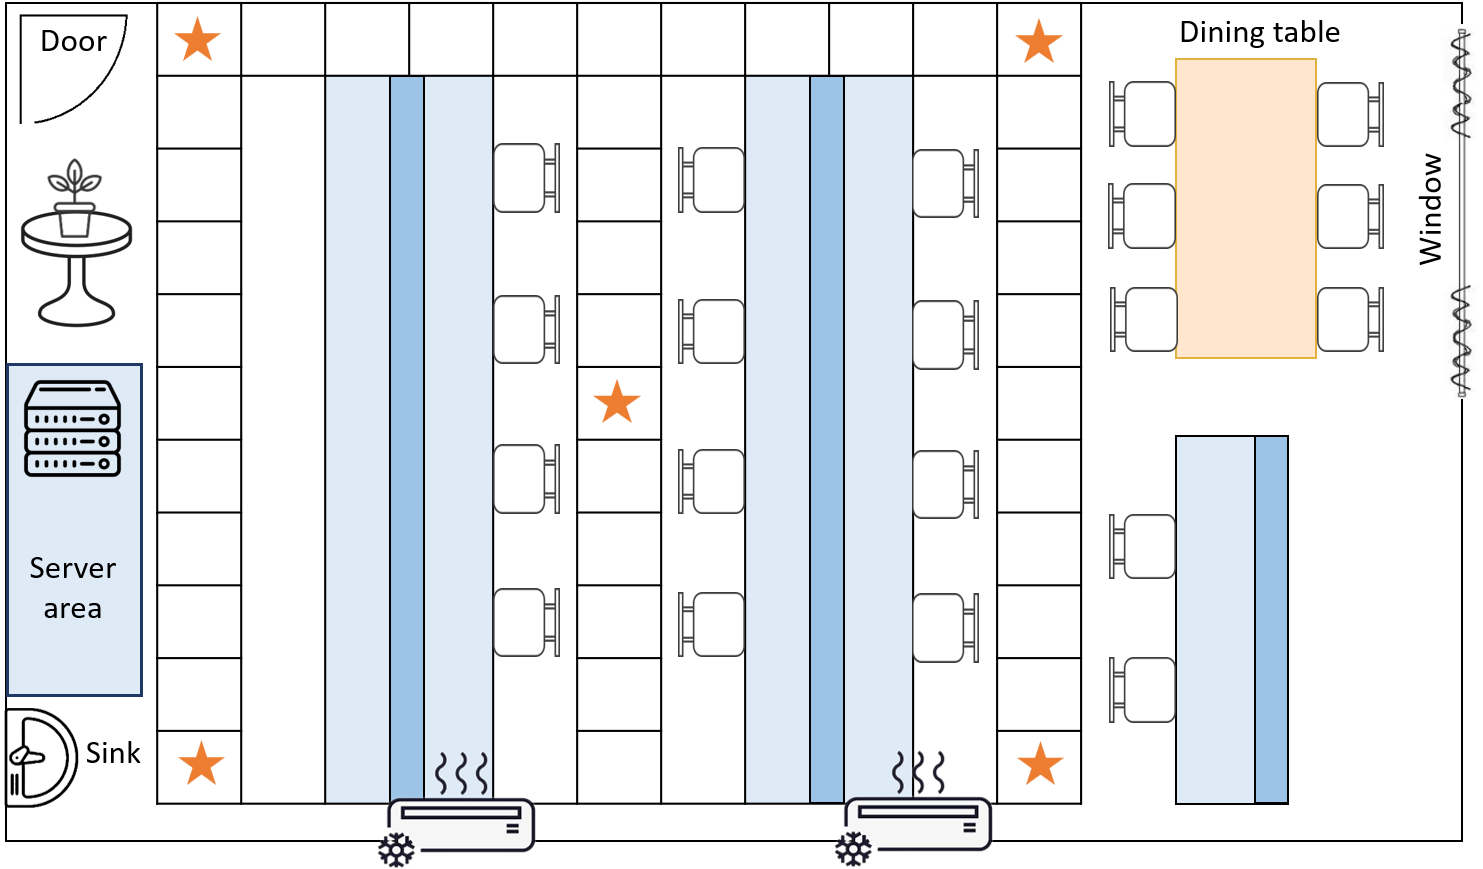
\includegraphics[width=\textwidth]{images/chap4/stationary.png}
        \end{minipage}
    }
    \subfloat[One of path of Scripted Walk]{
        \begin{minipage}[t]{0.48\columnwidth}
            \centering
            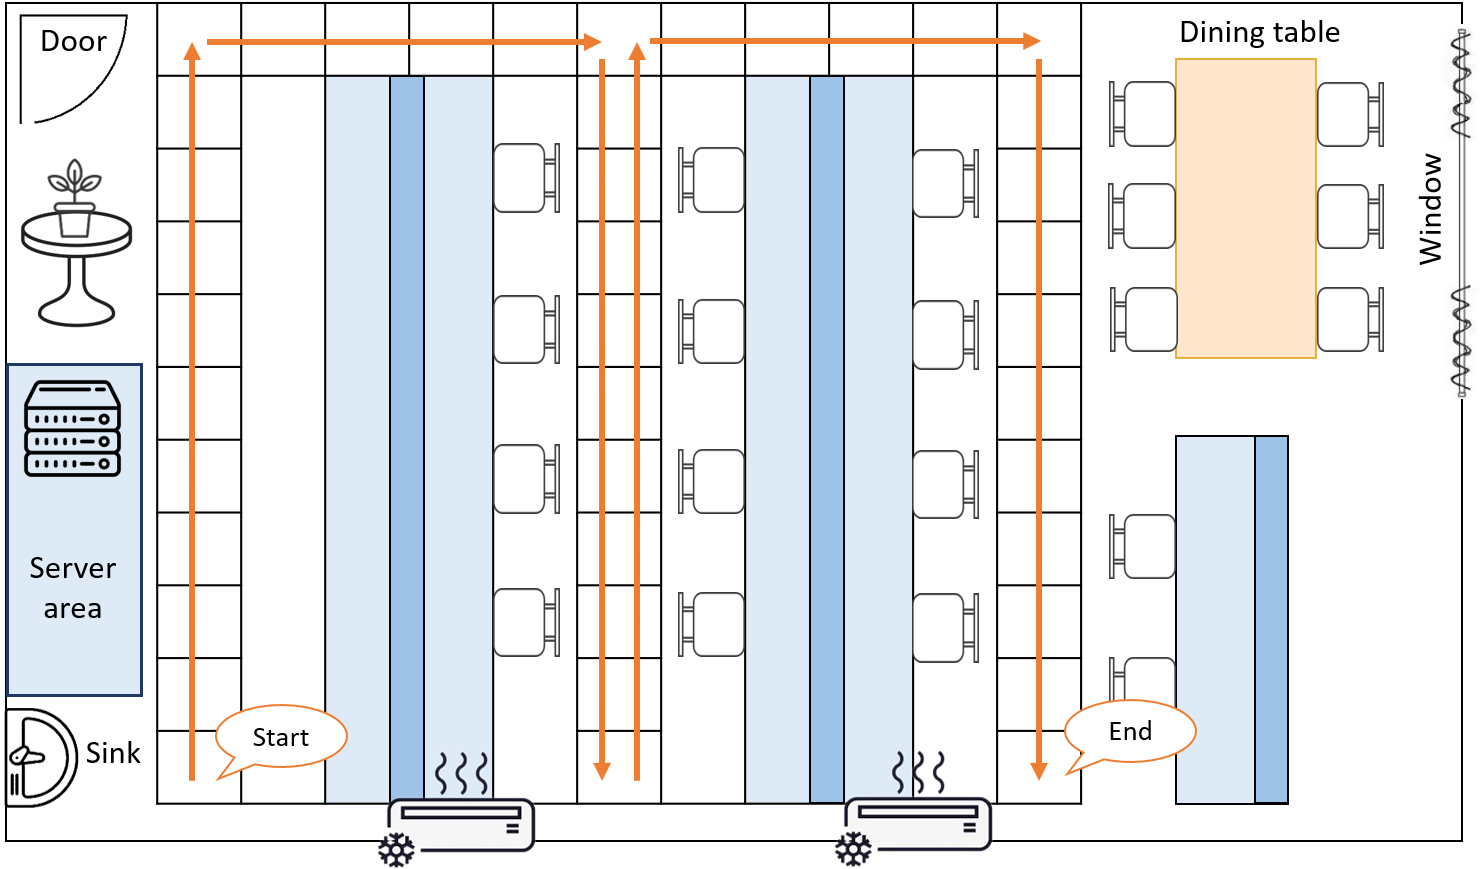
\includegraphics[width=\textwidth]{images/chap4/scripted.png}
        \end{minipage}
    }
    \caption{Definitions of Stationary and Scripted Walk.}
    \label{Fig:walk}
\end{figure}

\section{Experimental Datasets}
\paragraph{}
All data was collected in Room 92589 as mentioned above, including training dataset and test datasets. The training dataset was collected on March 18, 2022, while the two test datasets were collected at different times. The old test dataset was also collected on March 18, 2022, while the new test dataset was collected six months later, on October 28, 2022.
\begin{figure}[htbp]
    \centering
    \subfloat[March 18, 2022]{
        \begin{minipage}[t]{0.45\columnwidth}
            \centering
            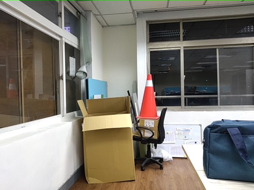
\includegraphics[width=0.9\textwidth]{images/chap4/old_scene.png}
        \end{minipage}
    }
    \subfloat[October 28, 2022]{
        \begin{minipage}[t]{0.45\columnwidth}
            \centering
            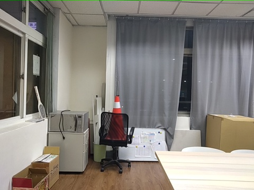
\includegraphics[width=0.9\textwidth]{images/chap4/new_scene.png}
        \end{minipage}
    }
    \caption{Photos token at the same location on different dates.}
    \label{Fig:scene}
\end{figure}

\paragraph{}
Through observation, we find that data collected at different times may have some differences in the images. There are many objects in the indoor space, and after a period of time, there are noticeable changes in the number, location, and type of objects, as shown in figure \ref{Fig:scene}. Although the images were taken at the same location, there are visible changes in the environment, such as the opening and closing of the curtains, the position of the cardboard boxes, and the appearance of the blue backpack. Additionally, we calculate the proportion of object categories in the old and new test datasets to understand the changes in the environment. Figure \ref{Fig:obj}. shows that while certain indoor essentials such as chairs, computer monitors, keyboards, and mice remained relatively constant in number, the quantity of some personal items like coffee mugs and backpacks varied. This shows that the indoor environment can change over time.
\begin{figure}[htbp]
    \centering
    \subfloat[Old test dataset]{
        \begin{minipage}[t]{0.8\columnwidth}
            \centering
            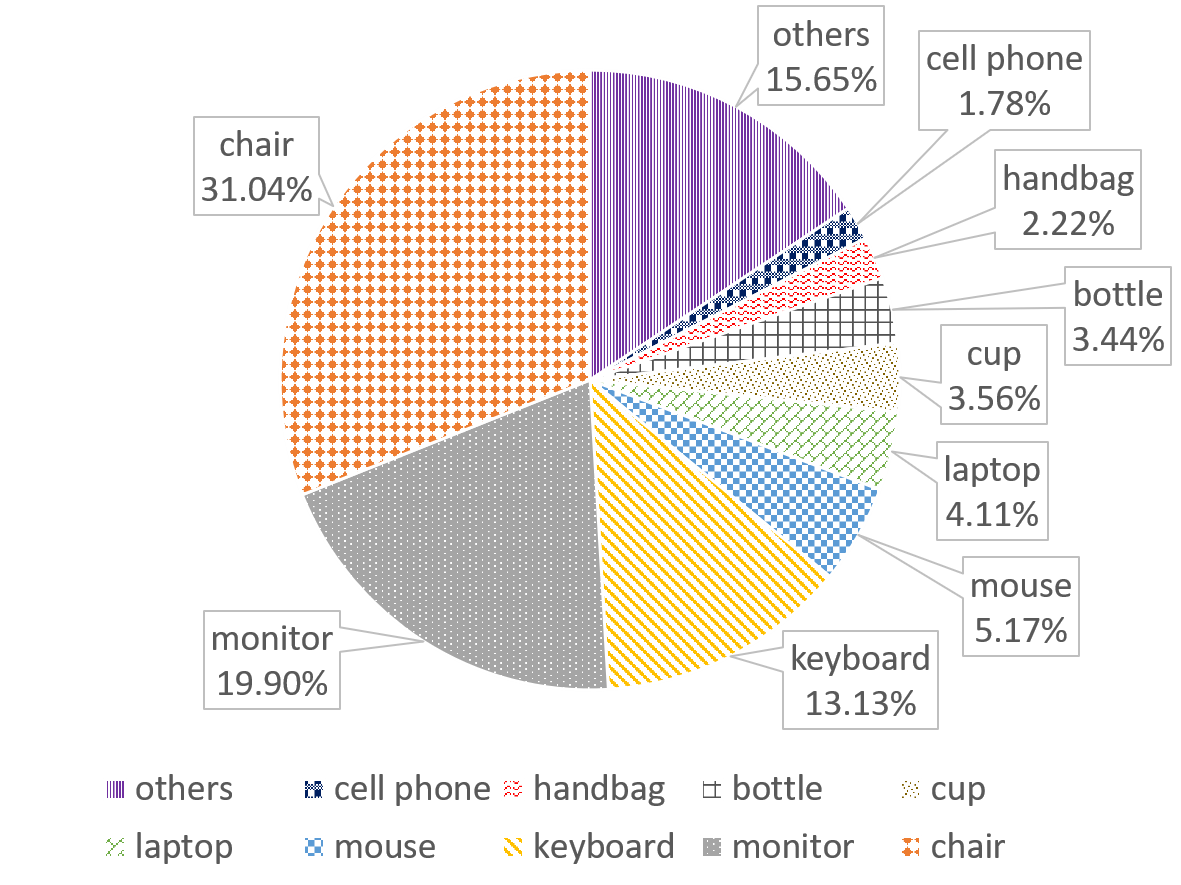
\includegraphics[width=\textwidth]{images/chap4/old_obj.png}
        \end{minipage}
    }
    
    \subfloat[New test dataset]{
        \begin{minipage}[t]{0.8\columnwidth}
            \centering
            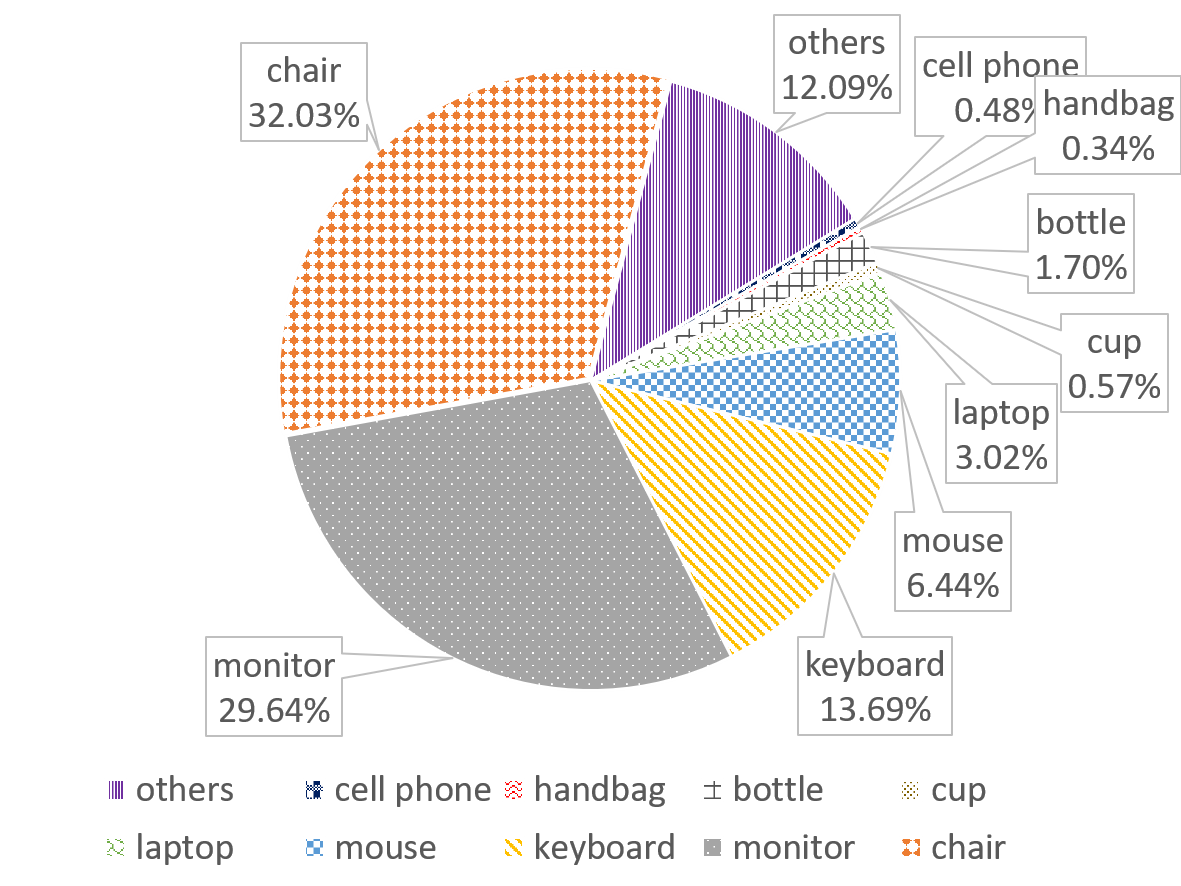
\includegraphics[width=\textwidth]{images/chap4/new_obj.png}
        \end{minipage}
    }
    \caption{Types of detected objects in old and new test dataset.}
    \label{Fig:obj}
\end{figure}

% ---------------- chapter 5 ----------------
\chapter{Performance Evaluation}
\paragraph{}
In this section, the results of different experiments will be presented. Here we use the mean distance error (MDE) and standard
deviation of the distance error (SDE) as the performance metric of the experiments. The formulas of MDE and SDE are defined as follow:
\begin{equation}
    \label{Eq:mde}
    MDE=\sum_i{\frac{\sqrt{(x_i-\hat{x_i})^2+(y_i-\hat{y_i})^2}}{N}}
\end{equation}
\begin{equation}
    SDE = \sqrt{\frac{\sum_{i}{(d_i-\bar{d})}^2}{N}}
\end{equation}
Where $x_i$, $y_i$ refer to the coordinate of the $i$-th estimated position and $\hat{x_i}$,$\hat{y_i}$ refer to the coordinate of the ground truth position. $N$ is the number of testing positions. Then $d_i$ means the distance errors between the $i$-th estimated position and its corresponding ground truth position, $\bar{d}$ is the mean of all $d_i$.
\paragraph{}
In the following section, we will compare our proposed method with other baseline methods as well as other multi-device systems on old test data. Additionally, we will apply the proposed method to a new test dataset to evaluate the effectiveness of data augmentation in adapting the system to dynamic environments. Finally, we will introduce challenging scenarios to the new dataset by introducing fake images and packet loss, aiming to validate the stability of our system.
% ---------------- section 5.1 ----------------
\section{Compare with Other Baseline Methods}
\paragraph{}
First, we compared our system with an existing method \cite{wang2020joint}, denoted as ``$Wang\ et\ al.$''. The system architecture of \cite{wang2020joint} is similar to ours, as both are hierarchical systems. However, the difference lies in the fact that \cite{wang2020joint} uses only wireless signals for coarse-grained positioning. Additionally, we also modified our system to compare the performance of using only wireless signals for coarse-grained positioning. The variation is denoted as ``Proposed $(W+I)$'', indicated that the use of wireless signals for coarse-grained positioning and images for fine-grained positioning.
\paragraph{}
The mean distance error (MDE) of all scenarios are show in Figure \ref{Fig:mde_baseline}. In the free walk scenario, our proposed system outperforms $Wang$ by at least $57\%$. In the scripted walk, the mean distance error improves $30\%$. Finally, we achieve a $70\%$ reduction in error in the stationary scenario. From the results, it can be observed that our system $Proposed(W+I)$ achieves better performance compared to $Wang\ et\ al.$ when utilizing the same data as input for the hierarchical framework. Moreover, our method $Proposed$ demonstrates superior performance. The detailed of MDE data is presented in the Table \ref{table:5_1_MDEs}.
\begin{figure}[h]
    \centering
    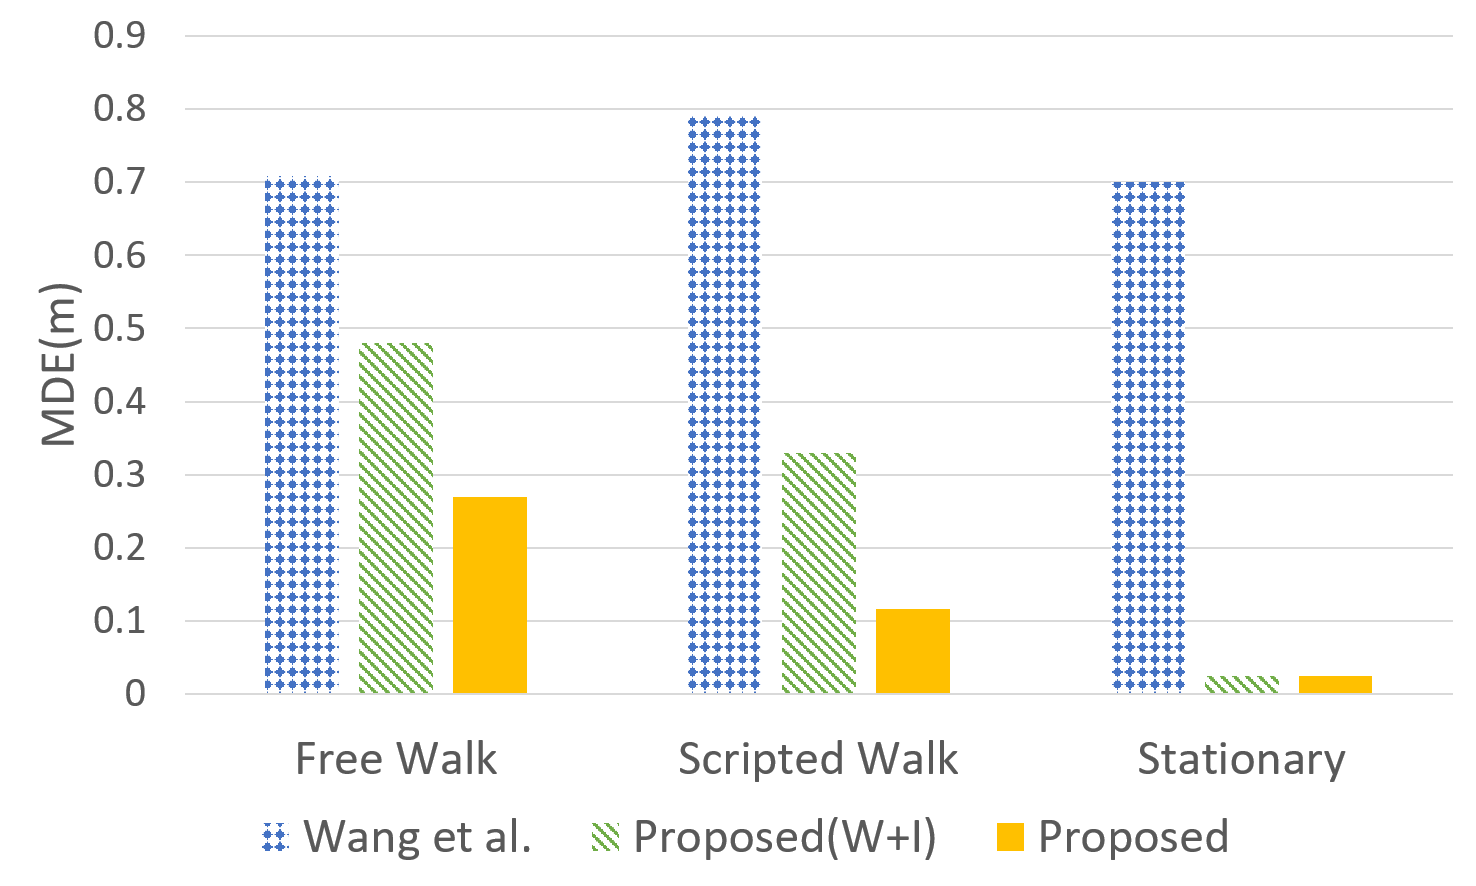
\includegraphics[width=0.8\columnwidth]{images/chap5-1/MDE_5-1.png}
    \caption{Comparisons of the proposed method with other baseline methods.}
    \label{Fig:mde_baseline}
\end{figure}
\begin{table}
    \begin{center}
    \caption{MDEs of proposed methods and baselines}
    \label{table:5_1_MDEs}
        \begin{tabular}{|c||c|c|c|c|}
            \hline
                Method & Free Walk & Scripted Walk & Stationary \\
            \hline
            \hline
                $Wang\ et\ al.$ & 0.709 m  & 0.792 m  & 0.7 m \\
            \hline
                $Proposed(W+I)$   & 0.48 m  & 0.33 m  & 0.025 m \\
            \hline
                $Proposed$   & 0.269 m & 0.116 m & 0.025 m \\
            \hline
        \end{tabular}
    \end{center}
\end{table}
\paragraph{}
Furthermore, we observed the MDE distributions of each method in each scenario. The cumulative distribution function (CDF) of each scenarios is shown in Figure \ref{Fig:cdf_baseline}. In the free walk (Figure \ref{Fig:cdf_baseline_fw}), $Wang\ et\ al.$ and $Proposed(W+I)$ have $90\%$ of the distance error less than $1.65$ (m) and $1.68$ (m) respectively. And the $90\%$ of the distance error of proposed method is $0.59$ (m). In the scenario of scripted walk (Figure \ref{Fig:cdf_baseline_sw}), $Wang$ and $Proposed(W+I)$ have $90\%$ of the distance error less than $1.78$ (m) and $1.13$ (m) respectively. And the $90\%$ of the distance error of proposed method is $0.49$ (m). In the scenario of stationary (Figure \ref{Fig:cdf_baseline_st}, please note that the CDF curves for $Proposed(W+I)$ and $Proposed$ overlap each other.), the $90\%$ of the distance error of $Wang\ et\ al.$ less than $1.8$ (m), while $Proposed(W+I)$ and $Proposed$ have distance error value $0$ (m). In summary, our proposed method consistently outperforms the baseline method in every scenario.
\begin{figure}[htbp]
    \centering
    \subfloat[CDF curve of free walk]{
        \begin{minipage}[t]{0.75\columnwidth}
            \centering
            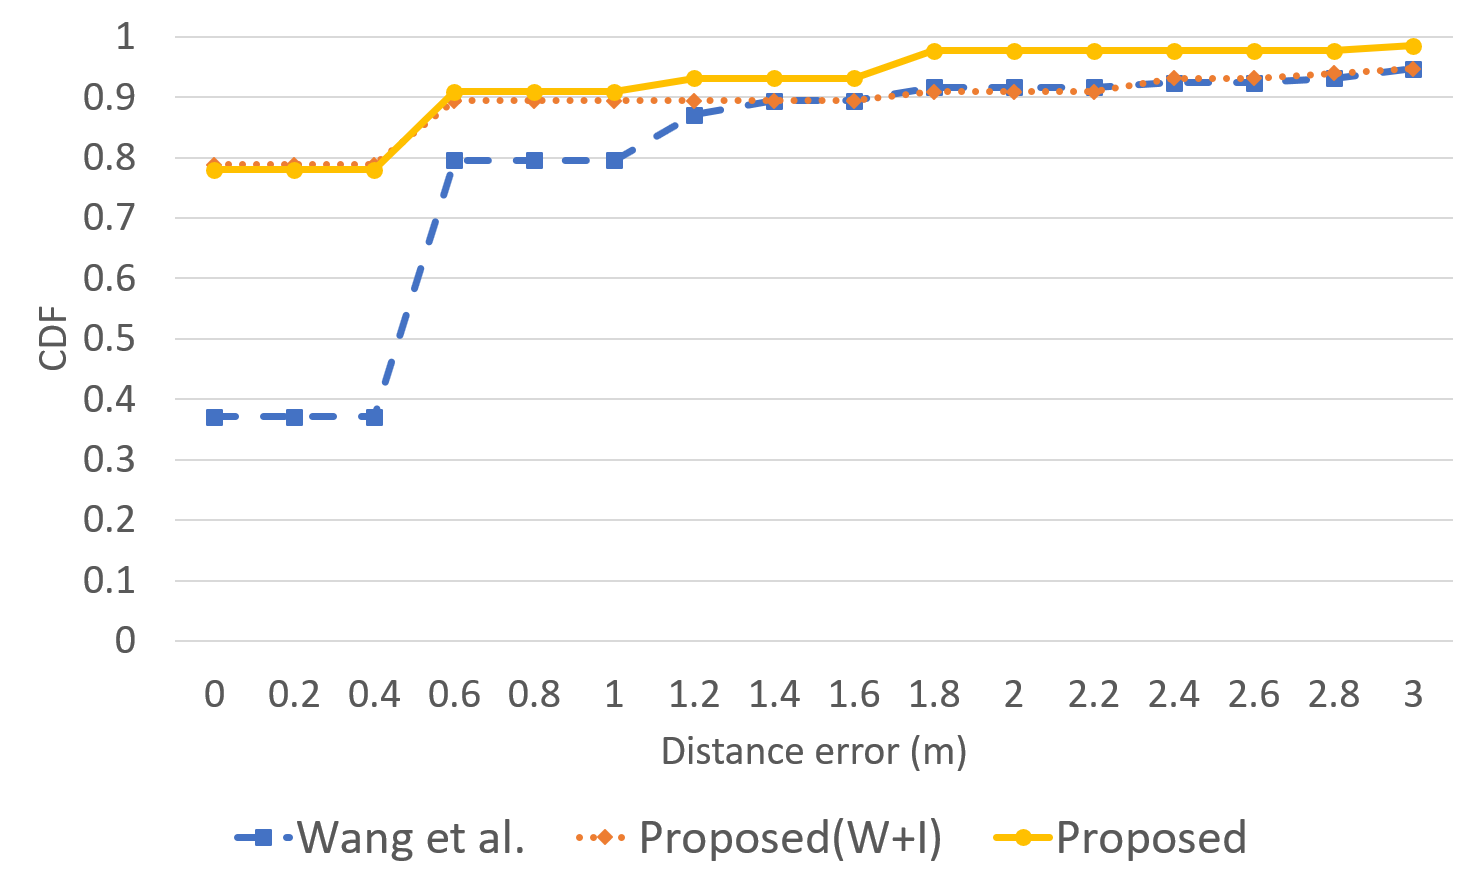
\includegraphics[width=0.9\textwidth]{images/chap5-1/CDF_FW_5-1.png}
            \label{Fig:cdf_baseline_fw}
        \end{minipage}
    }
    
    \subfloat[CDF curve of scripted walk]{
        \begin{minipage}[t]{0.75\columnwidth}
            \centering
            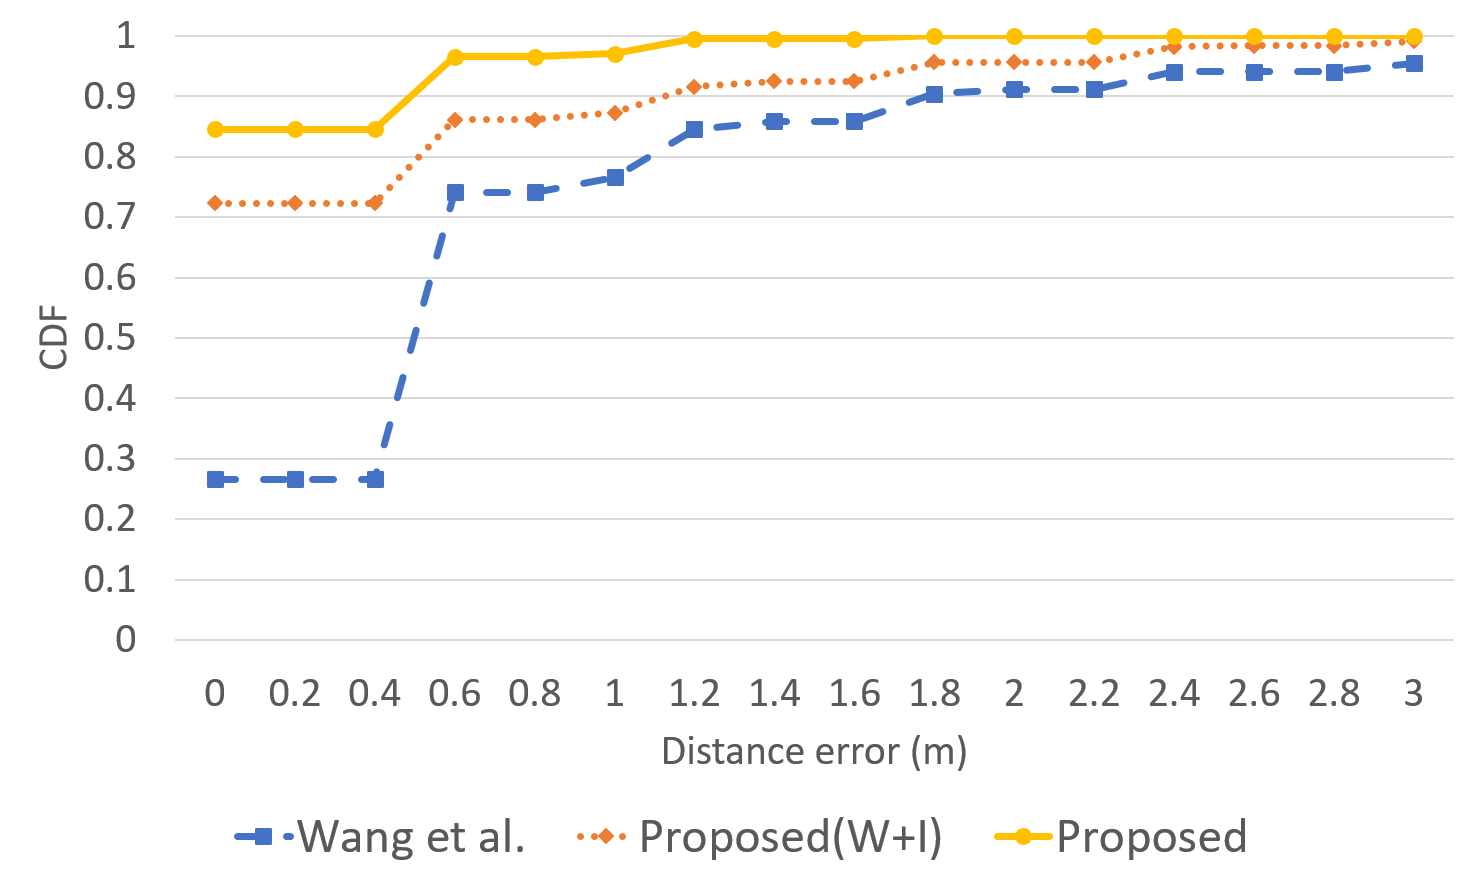
\includegraphics[width=0.9\textwidth]{images/chap5-1/CDF_SW_5-1.png}
            \label{Fig:cdf_baseline_sw}
        \end{minipage}
    }

    \subfloat[CDF curve of stationary]{
        \begin{minipage}[t]{0.75\columnwidth}
            \centering
            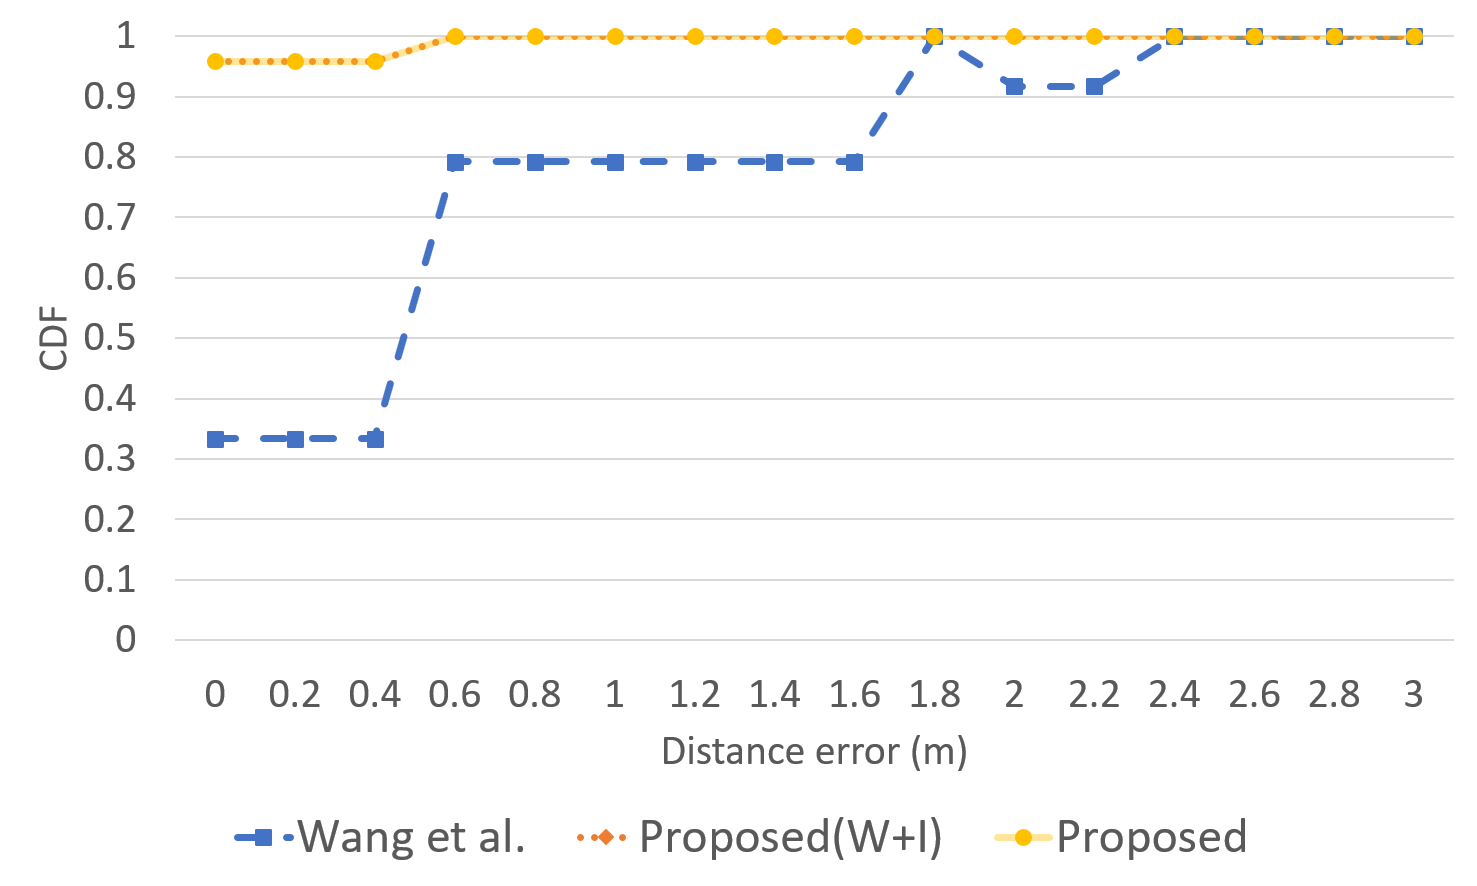
\includegraphics[width=0.9\textwidth]{images/chap5-1/CDF_ST_5-1.png}
            \label{Fig:cdf_baseline_st}
        \end{minipage}
    }
    \caption{Cumulative distribution function of the proposed method and other baseline methods in each scenario.}
    \label{Fig:cdf_baseline}
\end{figure}
% ---------------- section 5.2 ----------------
\section{Compare with Other Multi-device Systems}
\paragraph{}
Since our indoor positioning system can easily expand to multi-device architecture, we compare our work with other multi-device based indoor localization systems, $Lin's$ \cite{Lin2021} and $Wu's$ \cite{Wu2022}. Both of these methods are proposed for multi-device indoor positioning systems and utilize both wireless signals and visual data.
\begin{itemize}
    \item $Lin's$ \cite{Lin2021}: Obtain wireless and image fingerprint and using a multi-modal fusion algorithm to combine wireless and image data.
    \item $Wu's$ \cite{Wu2022}: Using wireless hash and image hash as fingerprints and proposed the dynamic weighting between wireless and image to respond to the immediate changes in the performance of both.
\end{itemize}
\paragraph{}
We conducted experiments using four mobile devices, similar to the methods proposed by $Lin's$ and $Wu's$. Each of the four devices captured images from different directions, including front, back, left, and right, as depicted in the Figure \ref{Fig:devices} and Table .
\begin{figure}[h]
    \centering
    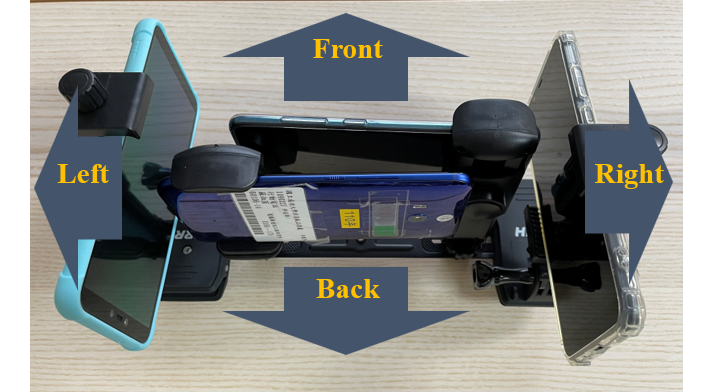
\includegraphics[width=0.8\columnwidth]{images/chap5-2/device.png}
    \caption{Experimental multi-devices.}
    \label{Fig:devices}
\end{figure}

\paragraph{}
Figure \ref{Fig:mde_multidevice} displays the MDE results and Table \ref{table:5_2_MDEs} shows the corresponding detailed numerical values. In the free walk scenario, our method achieved a minimum of $43\%$ reduction in error compared to the other two methods. In the scripted walk scenario, our method showed a significant improvement with an $87\%$ reduction in error. Furthermore, in the stationary scenario, our method achieved nearly error-free accuracy.
\begin{figure}[h]
    \centering
    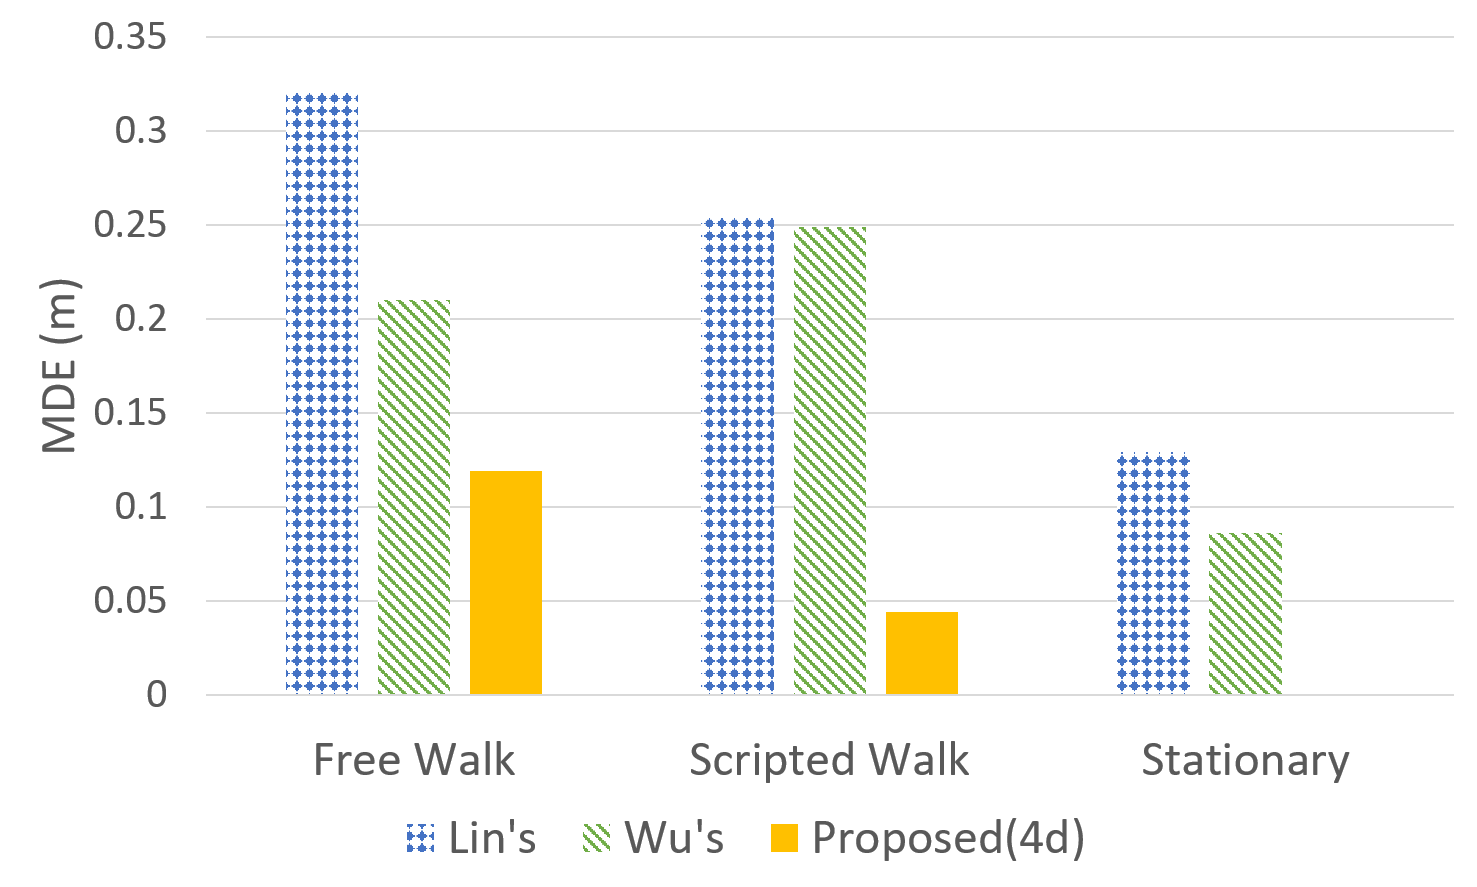
\includegraphics[width=0.8\columnwidth]{images/chap5-2/MDE_5-2.png}
    \caption{Comparisons of the proposed method with other multi-device systems.}
    \label{Fig:mde_multidevice}
\end{figure}
\begin{table}[htbp]
    \begin{center}
    \caption{MDEs of proposed methods and other multi-device systems}
    \label{table:5_2_MDEs}
        \begin{tabular}{|c||c|c|c|c|}
            \hline
                Method & Free Walk & Scripted Walk & Stationary \\
            \hline
            \hline
                $Lin's$ & 0.32 m  & 0.254 m  & 0.129 m \\
            \hline
                $Wu's$   & 0.21 m  & 0.249 m  & 0.086 m \\
            \hline
                $Proposed(4d)$    & 0.119 m & 0.044 m & 0.0 m \\
            \hline
        \end{tabular}
    \end{center}
\end{table}
\paragraph{}
Figure \ref{Fig:cdf_multidevice_fw} and Figure \ref{Fig:cdf_multidevice_sw} illustrate the CDF curves. In the free walk scenario, when calculating the $90\%$ distance error for each method, the errors for $Lin$ and $Wu$ are $1.04$ and $0.57$ meters, respectively, while our method achieves a $0.5$-meter distance error. Similarly, in the scripted walk scenario, when calculating the $90\%$ distance error for each method, the errors for $Lin$ and $Wu$  are $0.56$ and $0.58$ meters, respectively, while our method achieves a $0$-meter positioning error. From the CDF curves, it is evident that the proposed method consistently outperforms the other multi-device methods. Particularly, in the scripted walk scenario, our method significantly outperforms the other two methods.
\begin{figure}[htbp]
    \centering
    \subfloat[CDF curve of free walk]{
        \begin{minipage}[t]{0.75\columnwidth}
            \centering
            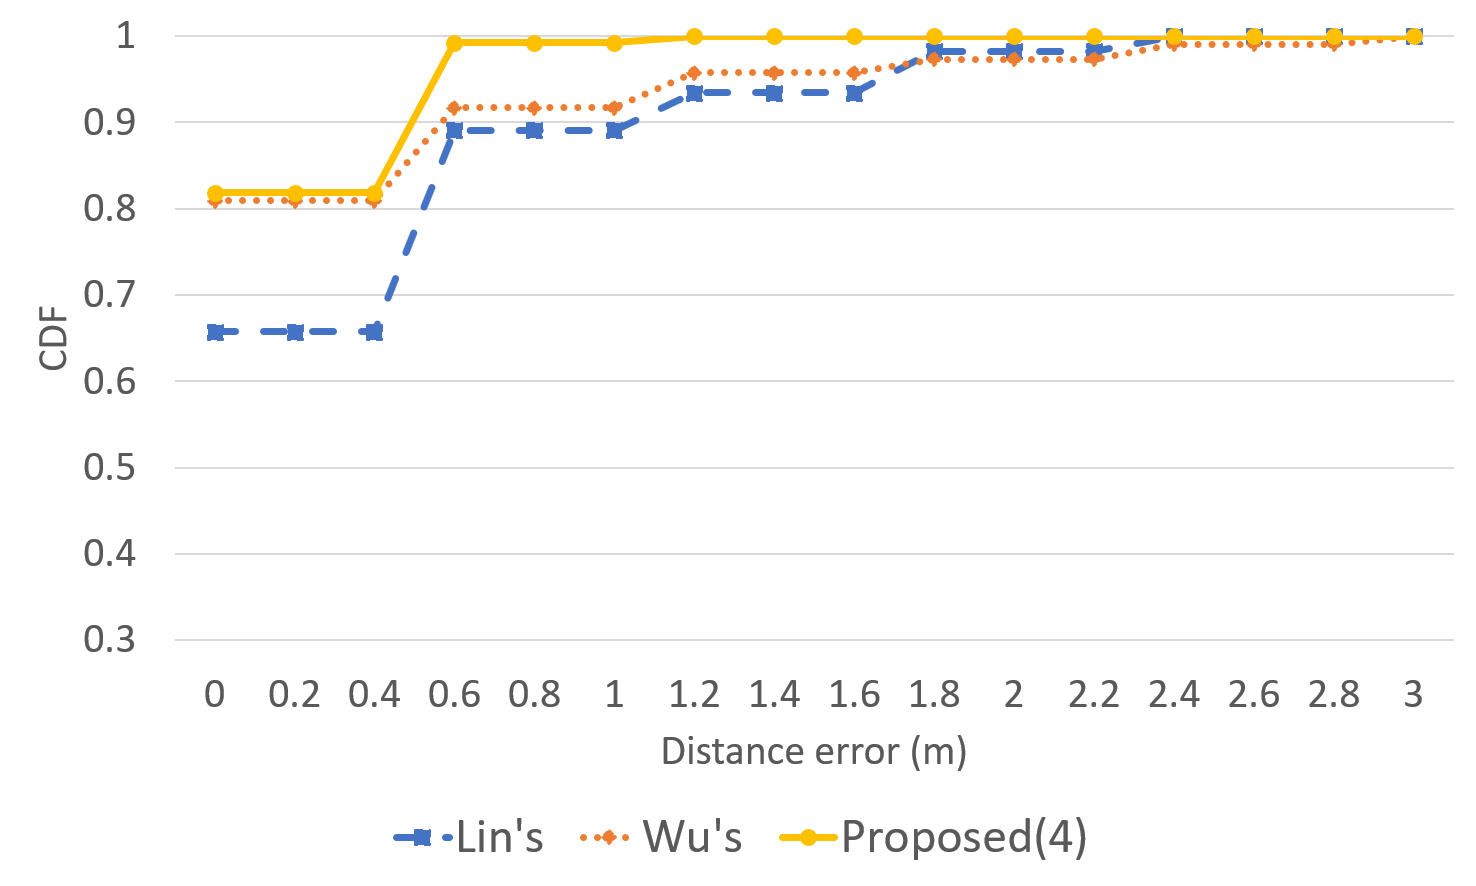
\includegraphics[width=0.9\textwidth]{images/chap5-2/CDF_FW_5-2.png}
            \label{Fig:cdf_multidevice_fw}
        \end{minipage}
    }
    
    \subfloat[CDF curve of scripted walk]{
        \begin{minipage}[t]{0.75\columnwidth}
            \centering
            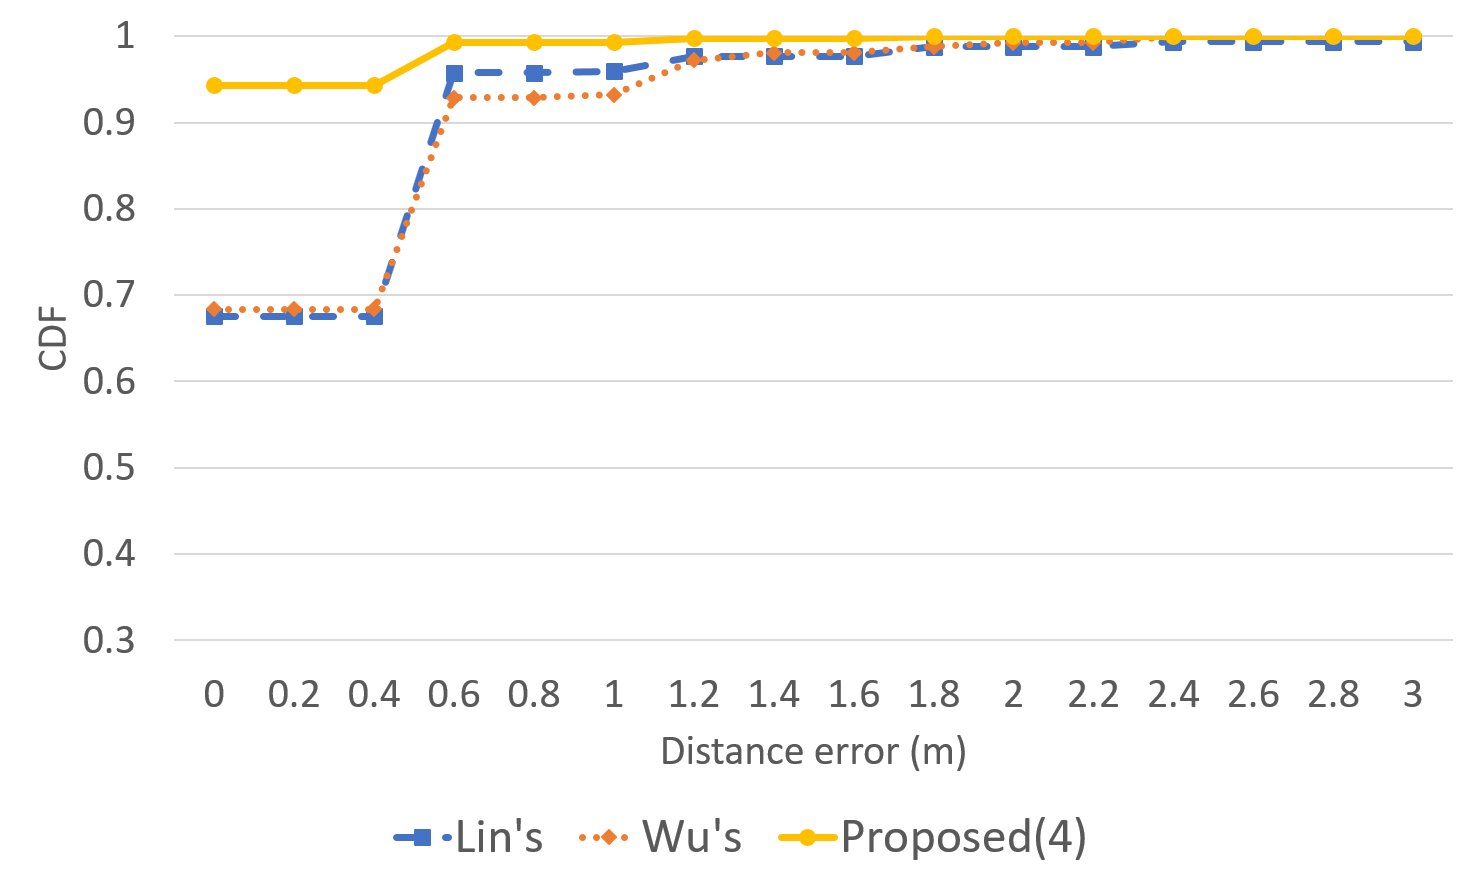
\includegraphics[width=0.9\textwidth]{images/chap5-2/CDF_SW_5-2.png}
            \label{Fig:cdf_multidevice_sw}
        \end{minipage}
    }
    \caption{Cumulative distribution function of the proposed method and other multi-device methods.}
    \label{Fig:cdf_multidevice}
\end{figure}
% ---------------- section 5.3 ----------------
\section{Contribution Between Wireless and Image}
\paragraph{}
This section explores the respective contributions of wireless and image to our positioning system.  To examine the contributions of wireless signals and images in our system, we adjusted the system to perform coarse-grained localization using only wireless signals or only images. For fine-grained localization, we maintained the use of images as input. These two methods are referred to as $Proposed(W+I)$ and $Proposed(I+I)$, respectively. Meanwhile, the term $Proposed(WI+I)$ represents the system that utilizes both wireless signals and images for coarse-grained localization.
\paragraph{}
Table \ref{table:5_3_MDEnSDE} displays the MDE and SDE values for each method in each scenario. Firstly, let's observe the performance of $Proposed(W+I)$ and $Proposed(WI+I)$. It can be observed that after incorporating images, there is a decreasing trend in both MDE and SDE values. This indicates that the inclusion of images enhances the localization accuracy of our system. Next, let's examine the performance of $Proposed (I+I)$ and $Proposed (WI+I)$. From the numerical values, it can be observed that after incorporating wireless signals, there is not a significant change in the MDE of the system. However, there is a substantial decrease in SDE. This suggests that the inclusion of wireless signals in the system helps mitigate larger distance errors.
\begin{table}[h]
    \begin{center}
    \caption{MDEs and SDEs between wireless and image of proposed system.}
    \label{table:5_3_MDEnSDE}
        \begin{tabular}{|c||c|c|c|c|c|c|}
            \hline
                & \multicolumn{2}{|c|}{Free Walk} & \multicolumn{2}{|c|}{Scripted Walk} & \multicolumn{2}{|c|}{Stationary}\\
            \hline
                Method & MDE & SDE & MDE & SDE & MDE & SDE \\
            \hline
            \hline
                $Proposed(W+I)$ & 0.48 m  & 1.226 m  & 0.33 m & 0.468 m & 0.025 m & 0.014 m \\
            \hline
                $Proposed(I+I)$   & 0.282 m  & 0.673 m  & 0.14 m & 0.202 m & 0.05 m & 0.027 m\\
            \hline
                $Proposed(WI+I)$    & 0.269 m & 0.384 m & 0.116 m & 0.084 m & 0.025 m & 0.014 m\\
            \hline
        \end{tabular}
    \end{center}
\end{table}
\paragraph{}
Overall, due to the capability of wireless signals to perform well in large-scale localization and their resistance to interference from similar scenes, they can effectively avoid significant positioning errors and provide more stable localization results. On the other hand, images are generally accurate for large-scale localization, thus improving the precision of localization. From the experimental results, it can be concluded that wireless signals and images contribute to different aspects of improvement (MDE and SDE). Therefore, using both types of data simultaneously for localization can lead to more accurate results.
% ---------------- section 5.4 ----------------
\section{Dynamic Indoor Environment Positioning}
\paragraph{}
Due to the fact that indoor environments can change over time, we collected a new set of test data in the same experimental space after a six-month interval. This new set of data, referred to as new test data, was used to evaluate the stability of our system. We compare the proposed method with and without data augmentation process, to confirm that the performance will more stable with data augmentation is applied.
\begin{table}[h]
    \begin{center}
    \caption{MDEs of the proposed system with and without data augmentation.}
    \label{table:5_3_MDEs}
        \begin{tabular}{|c||c|c|c|c|}
            \hline
                Method & Free Walk & Scripted Walk & Stationary \\
            \hline
            \hline
                $Proposed$ & 0.424 m  & 0.406 m  & 0.133 m \\
            \hline
                $Proposed(DA, 25\%)$   & 0.416 m  & 0.382 m  & 0.067 m \\
            \hline
                $Proposed(DA, 50\%)$    & 0.41 m & 0.328 m & 0.067 m \\
            \hline
                $Proposed(DA, 100\%)$    & 0.383 m & 0.346 m & 0.067 m \\
            \hline
        \end{tabular}
    \end{center}
\end{table}
\paragraph{}
The experimental results are depicted in the Figure \ref{Fig:mde_da}. In the figure, $Proposed(DA, mr)$ represents the proposed method with data augmentation, and the corresponding masking rate is indicated. For example, $Proposed (DA, 25\%)$ indicates that the proposed method incorporates data augmentation with a masking rate of $25\%$. From the experimental results, it can be observed that data augmentation leads to a decrease in mean distance error (MDE) in all experimental scenarios. In the free walk scenario, data augmentation results in an approximate decrease of 0.06 meters in MDE. In the scripted walk scenario, data augmentation leads to a reduction of approximately 0.08 meters in MDE. Furthermore, in the stationary scenario, data augmentation results in a $50\%$ decrease in MDE.
\begin{figure}[h]
    \centering
    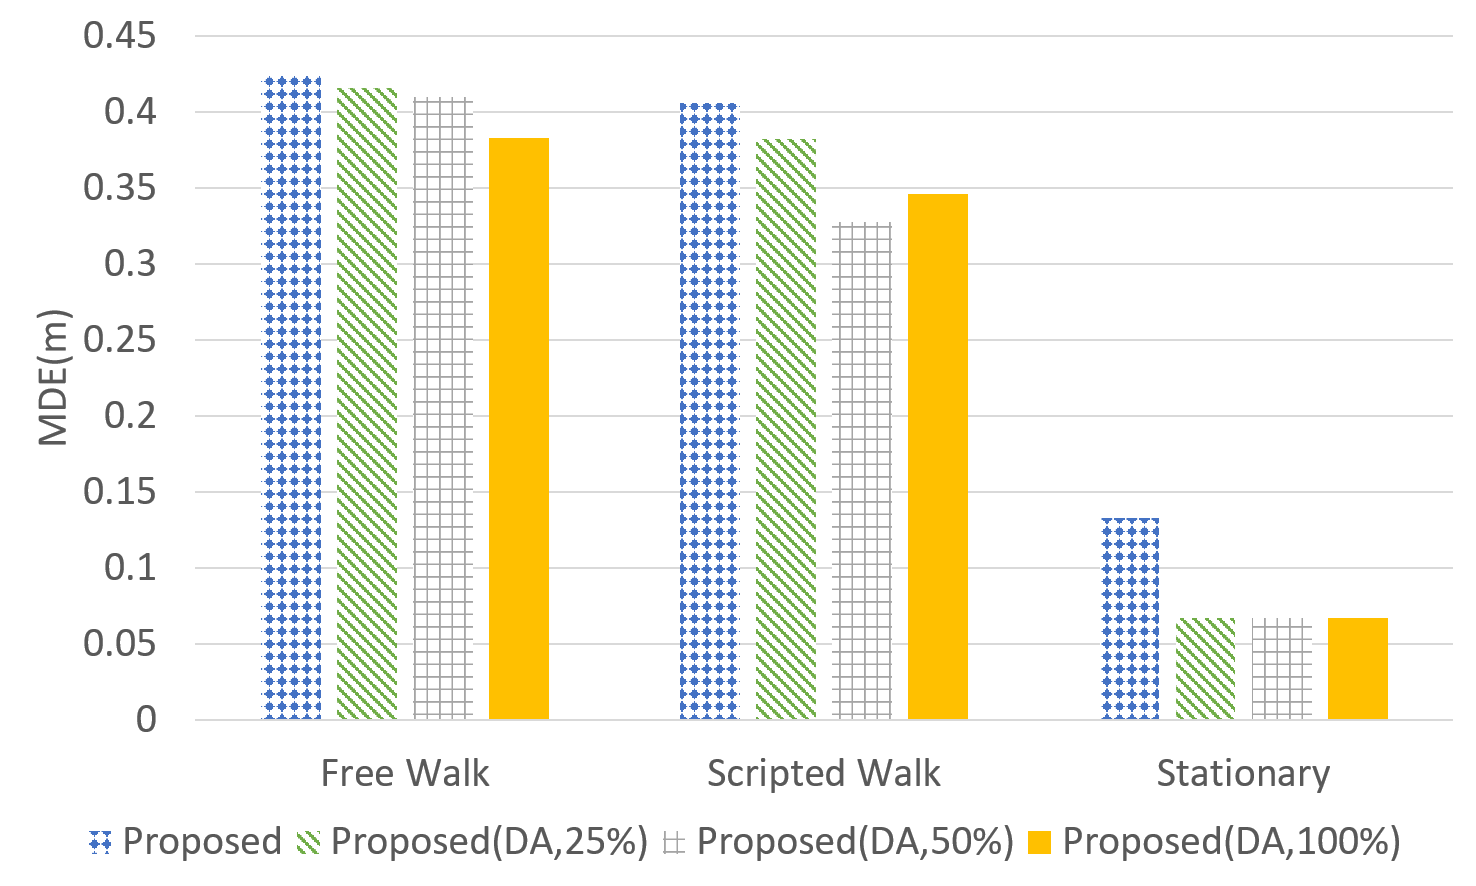
\includegraphics[width=0.8\columnwidth]{images/chap5-4/MDE_DA.png}
    \caption{MDE results of the proposed system with and without data augmentation.}
    \label{Fig:mde_da}
\end{figure}
% ---------------- section 5.5 ----------------
\section{Results of Fake and Missing Image Inputs}
\paragraph{}
As the mentioned before, the user can easily create the falsified image data during visual-based positioning. In this experiment, we simulated the scenario of falsified image data by replacing the original image data with images from different locations. As shown in Figure \ref{Fig:fake_walk}, users may create fake photos during their movement to confuse the positioning system. The experimental dataset we used was the new test dataset, which presented a greater challenge to the system. Therefore, through this experiment, we can validate the stability of our method under more challenging conditions.
\begin{figure}[h]
    \centering
    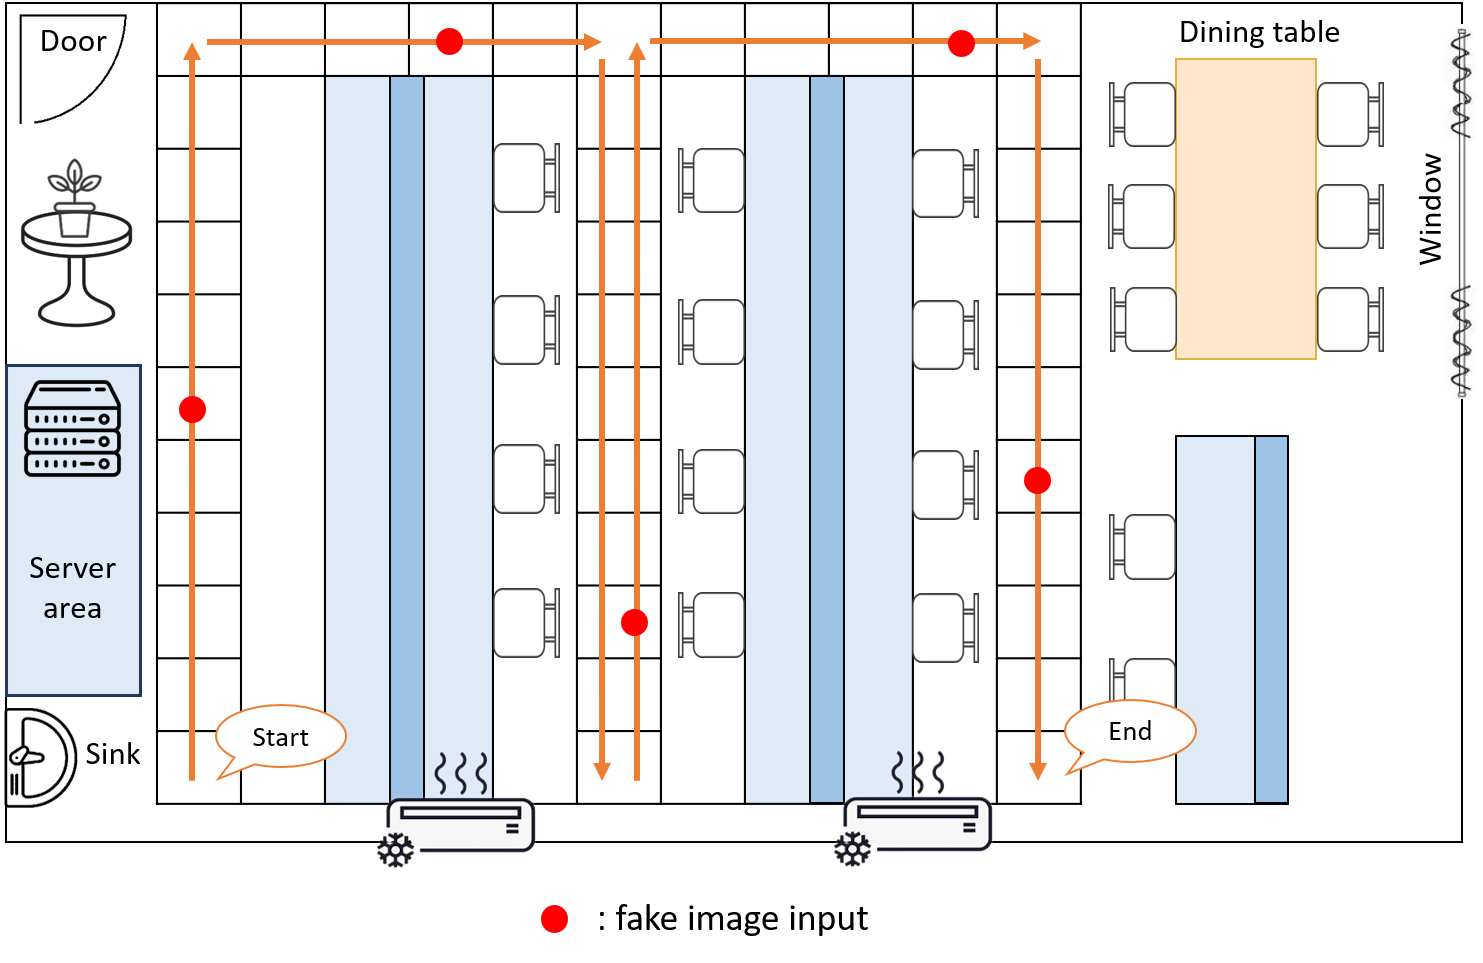
\includegraphics[width=0.7\columnwidth]{images/chap5-5/fake_walk.png}
    \caption{Experimental scenario with fake image inputs.}
    \label{Fig:fake_walk}
\end{figure}
\paragraph{}
The MDE results are shown in Figure \ref{Fig:fake_i}. From the figure, it can be observed that the introduction of fake images results in an increase in MDE, but it remains within the range of $0.7$ meters. Furthermore, the system with data augmentation still outperforms the system without data augmentation.
\begin{figure}[h]
    \centering
    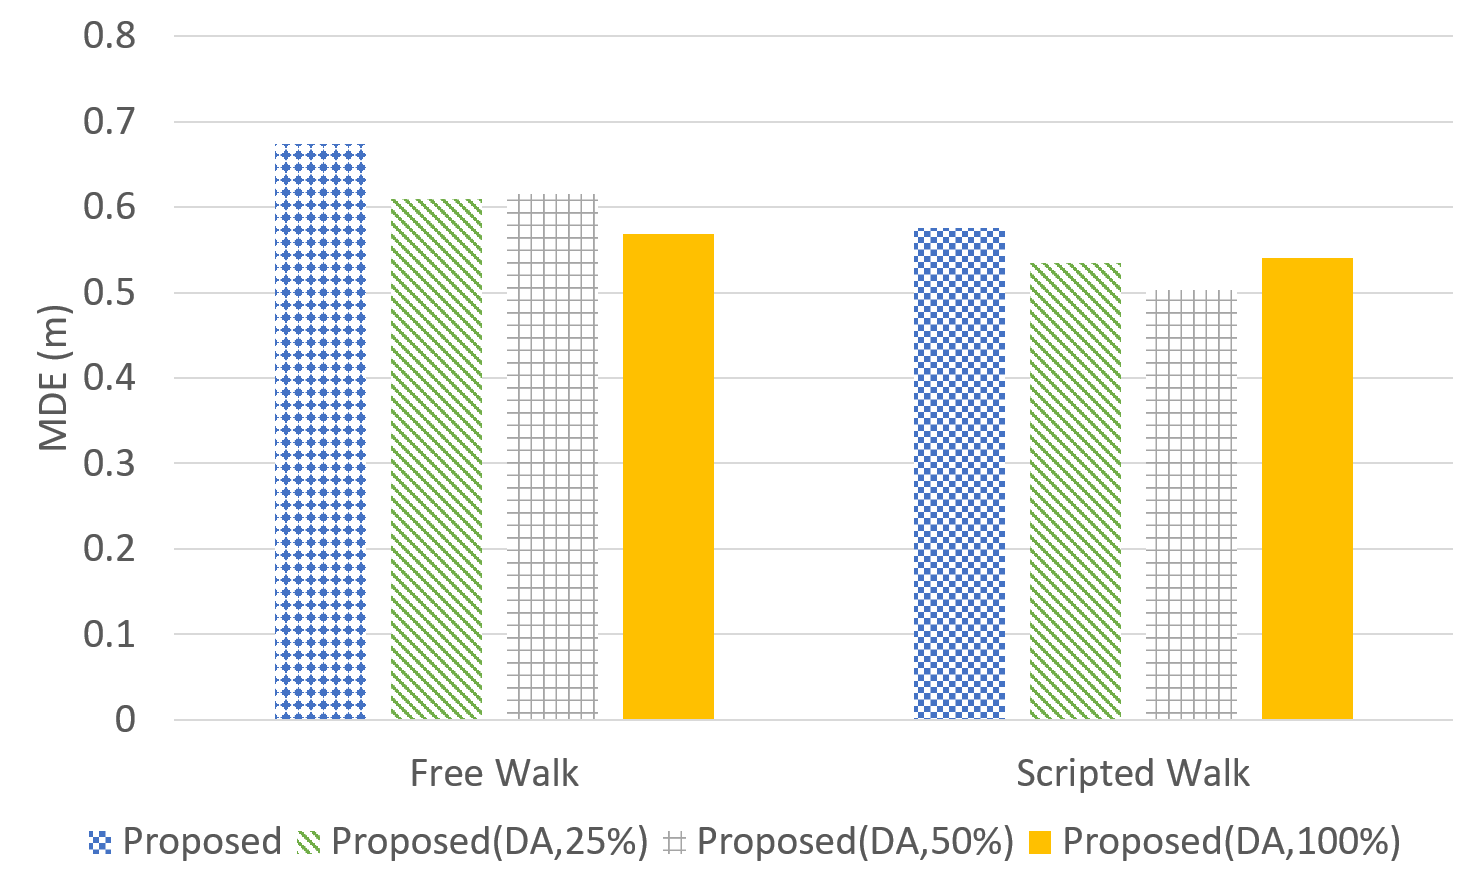
\includegraphics[width=0.65\columnwidth]{images/chap5-5/fake_i.png}
    \caption{MDE results of fake image inputs in free walk and scripted walk .}
    \label{Fig:fake_i}
\end{figure}
\paragraph{}
Furthermore, we also simulated the situation about missing image inputs. In this experiment, some samples will only retain wireless signal data as input. When an image is missing, our system can use the reference point predicted by the wireless signal in the W-space as a candidate for subsequent particle filter operations. The MDE results of missing image inputs are show in Figure \ref{Fig:missing_i}.
\begin{figure}[h]
    \centering
    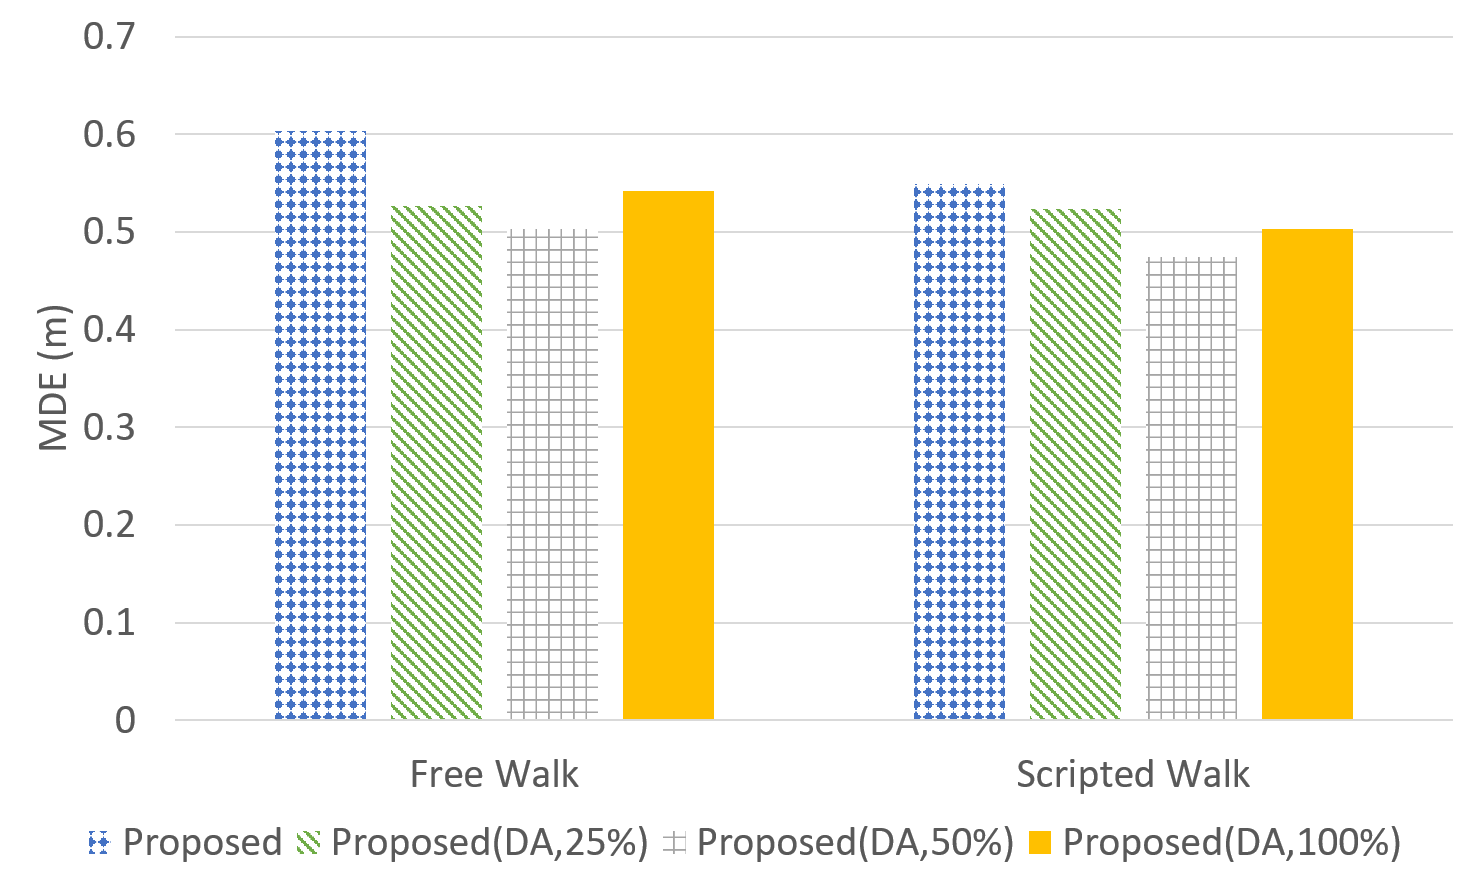
\includegraphics[width=0.65\columnwidth]{images/chap5-5/missing_i.png}
    \caption{MDE results of missing image inputs in free walk and scripted walk .}
    \label{Fig:missing_i}
\end{figure}
\paragraph{}
In the experiments, our system benefits from the W-space predicted by the wireless signal, which helps prevent significant distance errors when there are issues with the images. Additionally, the particle filter also plays a role in correcting positioning errors, especially when the user's movements follow a regular pattern. As a result, the error in the scripted walk scenario is lower than that in the free walk scenario.
% ---------------- section 5.6 ----------------
\section{Results of Signal Packet Loss}
\paragraph{}
In this experiment, we simulated packet loss scenarios. In randomly selected samples, we intentionally dropped certain packets to verify the impact of packet loss on our system. This allowed us to assess how packet loss affects the performance of our system. We also configured different percentages of packet loss scenarios, specifically $30\%$, $20\%$, and $10\%$. Similar to the previous experiment, we conducted the experiment using the new test dataset as well.
\paragraph{}
Figure \ref{Fig:fake_w} displays the experiment results. In this experiment, the MDE (Mean Distance Error) are consistently confined within $0.6$ meters, and the system with data augmentation performed better. With the assistance of image data and the particle filter, our system can maintain stability even in the presence of packet loss. 
\paragraph{}
\begin{figure}[htbp]
    \centering
    \subfloat[Free Walk]{
        \begin{minipage}[t]{0.7\columnwidth}
            \centering
            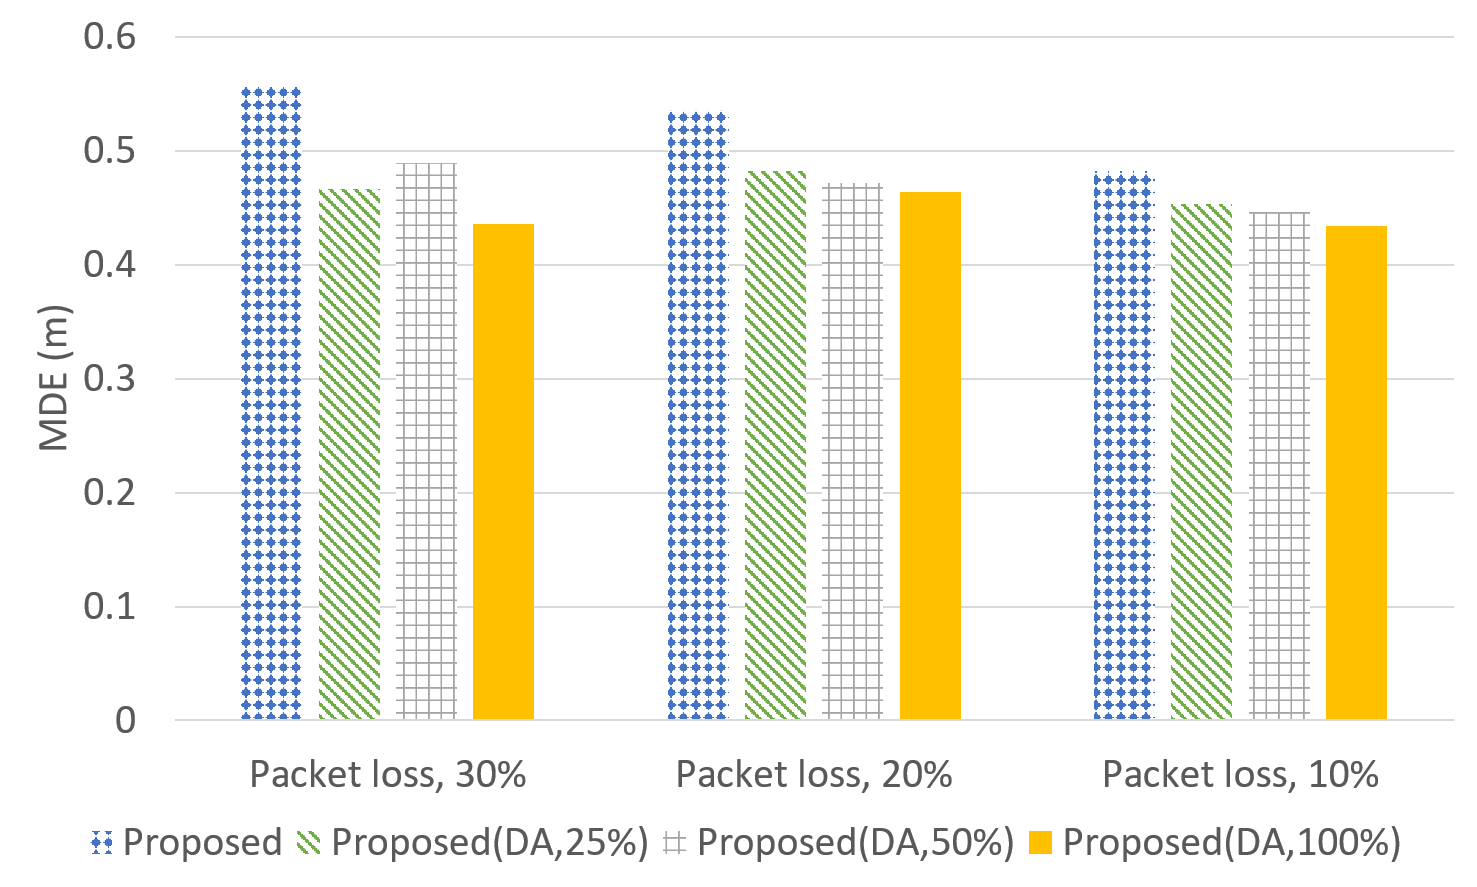
\includegraphics[width=\textwidth]{images/chap5-6/fake_w_FW.png}
        \end{minipage}
    }
    
    \subfloat[Scripted Walk]{
        \begin{minipage}[t]{0.7\columnwidth}
            \centering
            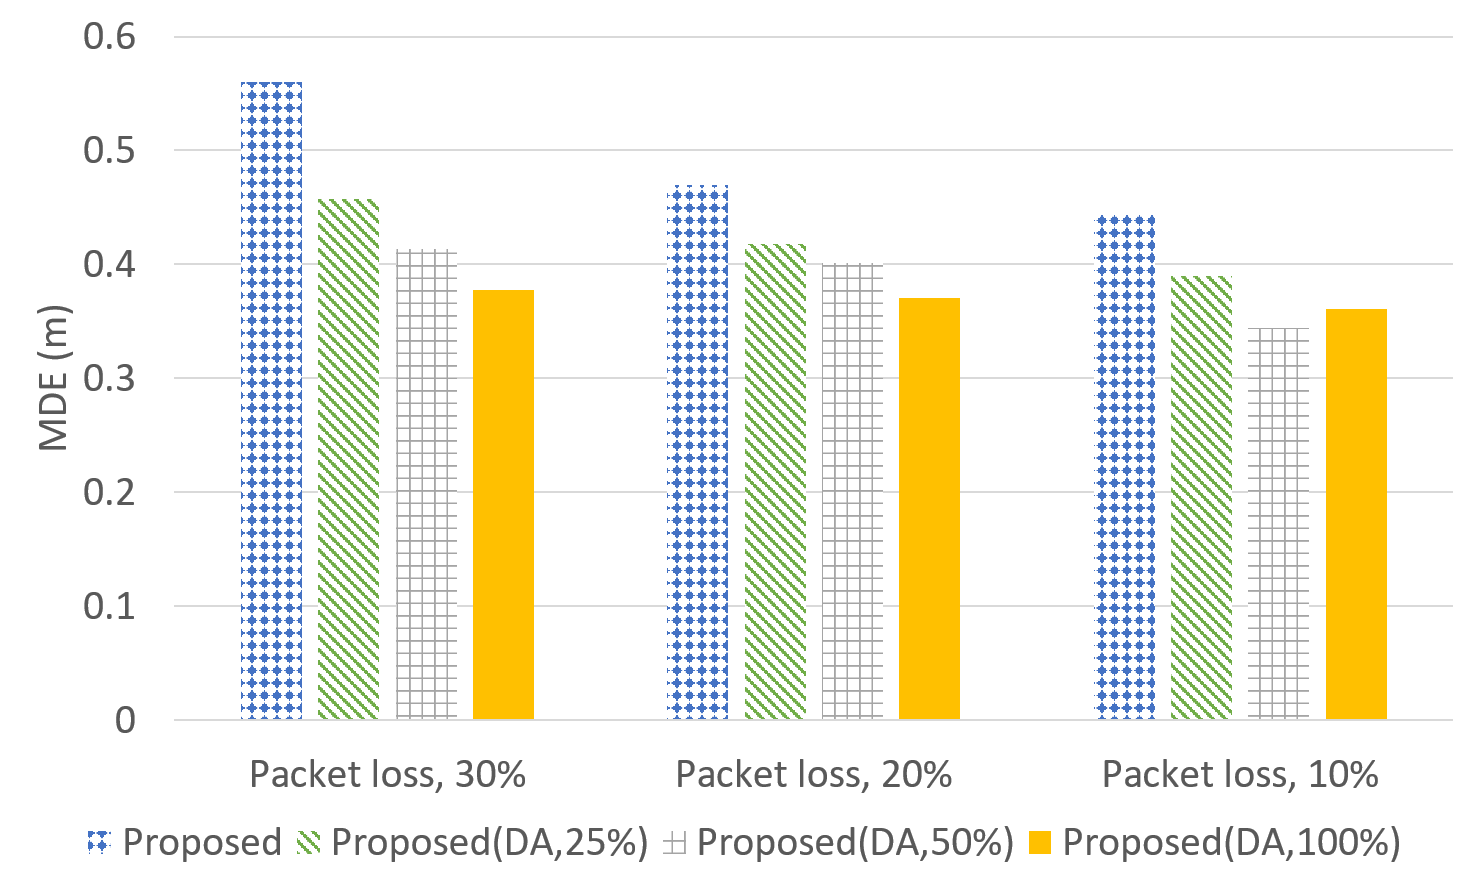
\includegraphics[width=\textwidth]{images/chap5-6/fake_w_SW.png}
        \end{minipage}
    }
    \caption{MDE results of signal packet loss experiment in different scenarios.}
    \label{Fig:fake_w}
\end{figure}

% ---------------- chapter 6 ----------------
\chapter{Conclusion}
\paragraph{}
In this paper, a hierarchical indoor positioning using wireless signals and images is proposed. We integrate the data based on their characteristics. In the coarse-grained localization stage, we utilize two types of data and propose an intuitive algorithm to enhance the reliability of this phase. Subsequently, in the fine-grained localization, we employ image data for precise positioning and employ a tree-structured image database to reduce search time. Finally, we calculate the novel input for the particle filter and apply it to track the user's location. Furthermore, to enable the system to adapt to dynamic indoor environments, we propose a novel data augmentation approach to enhance system stability.
\paragraph{}
Compared to similar methods, our system achieves a lower error of less than $0.3$ meters and, in the case of multiple devices, can achieve an error within $0.15$ meters. We collected a longitudinal dataset to validate that our system can adapt to dynamic indoor environments. Experimental results demonstrate that our system achieves an error within $0.4$ meters on the new test dataset. Lastly, to validate the stability of our system, we conducted experiments with fake and missing image inputs and signal packet loss on the new test dataset. The experimental results demonstrate that the error can be limited to within $0.7$ meters for fake image inputs and $0.6$ meters for signal packet loss.

\clearpage
\addcontentsline{toc}{chapter}{Bibliography}
\bibliographystyle{IEEEtran}
\bibliography{references}

\end{document}
